% =============================================================================================
% Phase I Project Progress Report -- NIT Warangal template format
% Compile with pdfLaTeX (Overleaf default):  latexmk -pdf main.tex
% =============================================================================================
\documentclass[12pt,a4paper,oneside]{report}
\usepackage{nitw-report}
% Display equations of report 45, re-typeset (numbered within chapters as in the original)
\newcommand{\EqThreeOne}{%
\begin{equation}
v(t)=\frac{y_{\text{base}}-y(x)}{82}\,\text{mV},\qquad t=\frac{x-x_0}{205.2}\,\text{s},
\label{eq:3.1}
\end{equation}}
\newcommand{\EqThreeTwo}{%
\begin{equation}
\begin{gathered}
\mathrm{ReLU}(x)=\max(0,x),\qquad \mathrm{SiLU}(x)=x\,\sigma(x),\qquad \mathrm{GELU}(x)=x\,\Phi(x),\\[4pt]
\text{h-swish}(x)=x\,\frac{\mathrm{ReLU6}(x+3)}{6},\qquad \sigma(x)=\frac{1}{1+e^{-x}},\\[4pt]
\mathrm{softmax}(\mathbf{z})_c=\frac{e^{z_c}}{\sum_{j=1}^{4}e^{z_j}},
\end{gathered}
\label{eq:3.2}
\end{equation}}
\newcommand{\EqThreeThree}{%
\begin{equation}
\hat{y}=\arg\max_k\, w_k P_k,\qquad
\mathbf{w}^{*}=\arg\max_{\mathbf{w}}\ \mathrm{Acc}(\mathbf{w})\ \ \text{s.t.}\ \ \min_k \mathrm{Rec}_k(\mathbf{w})\ge 0.18.
\label{eq:3.3}
\end{equation}}
\newcommand{\EqThreeFour}{%
\begin{equation}
t=\bar{d}\;\Big/\sqrt{\Big(\frac{1}{J}+\frac{n_2}{n_1}\Big)\hat{\sigma}_d^{2}},\qquad J=15.
\label{eq:3.4}
\end{equation}}

\numberwithin{equation}{chapter}

\begin{document}
% =============================================================================================
% Front matter, laid out exactly as the NITW Phase I template (title page, approval, certificate,
% declaration, acknowledgements, abstract, contents, lists).  Fill the [bracketed] fields.
% =============================================================================================
\newcommand{\ReportTitle}{Four-Class Left Ventricular Ejection Fraction Classification from 12-Lead ECG Printout Images using Foundation Models, Engineered ECG Features and Public-Data Transfer}
\newcommand{\ReportTitleUpper}{FOUR-CLASS LEFT VENTRICULAR EJECTION FRACTION CLASSIFICATION FROM 12-LEAD ECG PRINTOUT IMAGES USING FOUNDATION MODELS, ENGINEERED ECG FEATURES AND PUBLIC-DATA TRANSFER}
\newcommand{\StudentA}{Sai Chaithr}\newcommand{\RollA}{23ECB0A20}
\newcommand{\StudentB}{[Student 2 name]}\newcommand{\RollB}{[Roll No.]}
\newcommand{\StudentC}{[Student 3 name]}\newcommand{\RollC}{[Roll No.]}
\newcommand{\Guide}{[Guide's name with title]}
\newcommand{\GuideDesig}{[Designation]}
\newcommand{\Dept}{Electronics and Communication Engineering}
\newcommand{\DeptUpper}{ELECTRONICS AND COMMUNICATION ENGINEERING}
\newcommand{\Programme}{Electronics and Communication Engineering}
\newcommand{\MonthYear}{November 2026}

% spacing of the approval, certificate and declaration pages, calibrated to the template
\newlength{\apA}\setlength{\apA}{22.76pt}\newlength{\apB}\setlength{\apB}{86.91pt}\newlength{\apC}\setlength{\apC}{88.80pt}\newlength{\apD}\setlength{\apD}{88.80pt}
\newlength{\ceA}\setlength{\ceA}{38.18pt}\newlength{\ceB}\setlength{\ceB}{30.06pt}\newlength{\ceC}\setlength{\ceC}{99.58pt}\newlength{\ceD}\setlength{\ceD}{56.91pt}
\newlength{\deA}\setlength{\deA}{35.76pt}\newlength{\deB}\setlength{\deB}{10.01pt}\newlength{\deI}\setlength{\deI}{6.00pt}\newlength{\deS}\setlength{\deS}{2.00pt}\newlength{\deC}\setlength{\deC}{71.13pt}
\pagenumbering{roman}
% ---------------------------------------------------------------- title page (no number)
% vertical positions calibrated to the template's title page (1.1 line stretch; a longer title pushes the
% middle block down, the bottom block stays where it is)
\newlength{\tpTop}\setlength{\tpTop}{-28.20pt}
\newlength{\tpA}\setlength{\tpA}{25.61pt}     % title -> "Phase I ..."
\newlength{\tpIt}\setlength{\tpIt}{3.00pt}    % between the italic lines
\newlength{\tpB}\setlength{\tpB}{14.23pt}     % -> "of"
\newlength{\tpC}\setlength{\tpC}{11.38pt}     % -> "Bachelor of Technology"
\newlength{\tpD}\setlength{\tpD}{4.00pt}      % -> "in <programme>"
\newlength{\tpE}\setlength{\tpE}{11.38pt}     % -> "by"
\newlength{\tpF}\setlength{\tpF}{11.38pt}      % -> students
\newlength{\tpG}\setlength{\tpG}{7.41pt}    % between students
\newlength{\tpH}\setlength{\tpH}{17.64pt}     % -> "Under the guidance of"
\newlength{\tpI}\setlength{\tpI}{8.54pt}      % -> guide
\newlength{\tpJ}\setlength{\tpJ}{-0.00pt}      % -> designation
\newlength{\tpK}\setlength{\tpK}{8pt}      % -> logo
\newlength{\tpL}\setlength{\tpL}{3.00pt}      % department -> NITW
\newlength{\tpM}\setlength{\tpM}{3.00pt}      % NITW -> date
\newlength{\tpBottom}\setlength{\tpBottom}{0.00pt}
\begin{titlepage}
\setstretch{1.1}
\begin{center}
\vspace*{\tpTop}
{\Large\bfseries\ReportTitleUpper\par}
\vspace{\tpA}
{\bfseries\itshape Phase I Project Progress Report submitted to the\\[\tpIt]
National Institute of Technology Warangal\\[\tpIt]
in partial fulfilment of the requirements for the award of the degree\par}
\vspace{\tpB}
{\bfseries\itshape of\par}
\vspace{\tpC}
{\large\bfseries Bachelor of Technology\\[\tpD] in \Programme\par}
\vspace{\tpE}
{\bfseries\itshape by\par}
\vspace{\tpF}
{\large\bfseries \StudentA}\ (Roll No.\ \RollA)\\[\tpG]
{\large\bfseries \StudentB}\ (Roll No.\ \RollB)\\[\tpG]
{\large\bfseries \StudentC}\ (Roll No.\ \RollC)\par
\vspace{\tpH}
Under the guidance of\par
\vspace{\tpI}
{\large\bfseries \Guide\par}
\vspace{\tpJ}
{\small \GuideDesig, Department of \Dept\par}
\vspace{\tpK}

\includegraphics[width=2.3cm]{figures/nitw_logo.png}\par
\vfill
{\bfseries DEPARTMENT OF \DeptUpper\\[\tpL]
NATIONAL INSTITUTE OF TECHNOLOGY WARANGAL\\[\tpM]
\MonthYear\par}
\vspace{\tpBottom}
\end{center}
\end{titlepage}
\setcounter{page}{2}

% ---------------------------------------------------------------- approval of the project evaluation board
\thispagestyle{empty}
\addcontentsline{toc}{chapter}{Certificate of Approval}
{\centering\large\bfseries APPROVAL OF THE PROJECT EVALUATION BOARD\par}
\vspace{30pt}
\hfill DD/MM/YYYY\hspace*{\fontdimen2\font}\par   % template keeps one word space after the date
\vspace{\apA}
Certified that the report entitled \textbf{\ReportTitle} submitted by \StudentA\ (Roll No.\ \RollA), \StudentB\ (Roll No.\ \RollB) and \StudentC\ (Roll No.\ \RollC) to the National Institute of Technology Warangal, as the Phase I progress report of their Bachelor of Technology project in \Programme, has been examined and accepted by the evaluation board.

\vspace{\apB}
\noindent(Member of the Board)\hfill(Member of the Board)\hfill(Member of the Board)

\vspace{\apC}
\noindent(Supervisor)\hfill(Co-Supervisor)

\vspace{\apD}
\noindent(Head of the Department)\hfill(Chairperson, Evaluation Board)
\clearpage

% ---------------------------------------------------------------- certificate
\thispagestyle{empty}
\addcontentsline{toc}{chapter}{Certificate}
{\centering (The certificate is to be printed on the Departmental Letter-Head)\par}
\vspace{\ceA}
{\centering\large\bfseries\underline{CERTIFICATE}\par}
\vspace{\ceB}
\noindent This is to certify that the report entitled \textbf{\ReportTitle}, submitted by \textbf{\StudentA\ (Roll No.\ \RollA), \StudentB\ (Roll No.\ \RollB) and \StudentC\ (Roll No.\ \RollC)} to the National Institute of Technology Warangal, is a record of bona fide project work carried out by them under my (our) supervision during Phase I of their Bachelor of Technology project in \Programme.

\vspace{\ceC}
\noindent\begin{tabular}{@{}c@{}}
\rule{6cm}{0.4pt}\\
Supervisor\\
\Guide
\end{tabular}

\vspace{\ceD}
\noindent Date:
\clearpage

% ---------------------------------------------------------------- declaration
\thispagestyle{empty}
\addcontentsline{toc}{chapter}{Declaration}
{\centering\large\bfseries DECLARATION\par}
\vspace{\deA}
\noindent We certify that
\begin{enumerate}[label=\alph*.,leftmargin=2em,topsep=\deB,itemsep=\deI]
  \item The work contained in the report is original and has been done by us under the general supervision of our supervisor(s).
  \item The work has not been submitted to any other Institute for any degree or diploma.
  \item We have followed the guidelines provided by the Institute in writing the report.
  \item Whenever we have used materials (data, theoretical analysis, and text) from other sources, we have given due credit to them by citing them in the text of the report and giving their details in the references.
  \item Whenever we have quoted written materials from other sources, we have put them under quotation marks and given due credit to the sources by citing them and giving required details in the references.
  \item We took help from an AI assistant for some tasks, such as writing and checking code, running the documented experiments and checking the wording. All design decisions, data handling approvals and conclusions are our own.
\end{enumerate}

\vspace{\deC}
\noindent\begin{tabular}{@{}c@{\hspace{35.1pt}}c@{\hspace{35.1pt}}c@{}}
\rule{4.2cm}{0.4pt} & \rule{4.2cm}{0.4pt} & \rule{4.2cm}{0.4pt}\\
\StudentA & \StudentB & \StudentC\\
(\RollA) & (\RollB) & (\RollC)
\end{tabular}\par
\vspace{\deS}
{\centering Signatures of the Students\par}
\clearpage

% ---------------------------------------------------------------- acknowledgements (moved here from the end, as in the template)
\thispagestyle{empty}
\addcontentsline{toc}{chapter}{Acknowledgements}
\frontheading{Acknowledgements}
We thank our supervisor, \Guide, for guidance throughout Phase I, and the Department of \Dept, National Institute of Technology Warangal, for its support. We thank the cardiology department of the partner hospital for the ECG and echocardiography records, and the creators of EchoNext, ECGFounder and the other open resources used in this work.

\vspace{24pt}
\hfill\textbf{\StudentA, \StudentB\ and \StudentC}
\clearpage

% ---------------------------------------------------------------- abstract
\fancyhead[L]{}\fancyhead[R]{\thepage}
\addcontentsline{toc}{chapter}{Abstract}
\frontheading{Abstract}
Heart failure with reduced left ventricular ejection fraction (LVEF) is common and treatable but often detected late, because echocardiography is not available at every point of care. The 12-lead ECG is recorded routinely, yet in many Indian hospitals it survives only as a printed PDF page. This project grades LVEF into four classes (Normal, Mild, Moderate, Severe) from such printout images alone.

The data are 1,047 single-centre printouts from 993 patients, labelled from echocardiography: 837 ECGs for development and 210 locked until the final model was frozen. The traces were recovered exactly from the vector PDFs. Every model was evaluated with patient-grouped, repeated, nested cross-validation, corrected intervals and a written pre-registration. More than 1,300 results were recorded across ten stages, covering image CNNs, the ECGFounder and ECG-FM foundation models, LSTM and CNN-LSTM networks, 594 engineered features, gradient boosting, staged and ordinal ensembles and triage prediction. The public EchoNext data (4,827 ECGs) were redrawn in the hospital format and used for transfer learning.

The best four-class accuracy on all patients, from image-derived inputs only, is 0.587 [0.565, 0.610], above the model that also reads the printed machine measurements (0.562) and the original image CNN (0.471). A triage model that answers only confident cases is correct for 0.694 of the 56\,\% of patients it answers in cross-validation and 0.747 of the 50\,\% it answers on the locked test, scored once. Models trained only on EchoNext detect EF $\le 45$\,\% on the hospital printouts with AUROC 0.85. A simulation shows why all model families converge near 0.59: the ECG-based EF estimate correlates with echo at $r\approx0.66$, and 0.70 on all patients would need $r\approx0.90$. Phase II will use digital ECGs, larger linked datasets and verified Simpson-method EF labels.

\textbf{Index Terms:} electrocardiogram, left ventricular ejection fraction, heart failure screening, ECG printout digitisation, ECG foundation model, ECGFounder, EchoNext, transfer learning, ensemble learning, selective prediction, nested cross-validation.
\clearpage
\fancyhead[L]{\nouppercase{\leftmark}}\fancyhead[R]{\thepage}

% ---------------------------------------------------------------- contents and lists
\renewcommand{\contentsname}{Contents}
\begingroup\setstretch{\liststretch}
\tableofcontents
\clearpage
\phantomsection\addcontentsline{toc}{chapter}{List of Figures}
\listoffigures
\clearpage
\phantomsection\addcontentsline{toc}{chapter}{List of Tables}
\listoftables
\clearpage
\endgroup

% ---------------------------------------------------------------- abbreviations and notation
% template: \LARGE heading, running header, list at 1.2 stretch, indented 18 pt, abbreviation column 2.6 cm
\clearpage
\begingroup\setstretch{\liststretch}
\thispagestyle{fancy}
\markboth{List of Abbreviations}{}
\phantomsection\addcontentsline{toc}{chapter}{List of Abbreviations}
\frontheading{List of Abbreviations}
\vspace*{7pt}%                     template: the list starts 7 pt lower than body text under a heading
\newcommand{\abbrtable}[1]{\noindent\hspace*{18pt}\begin{tabular}{@{}>{\raggedright\arraybackslash}p{2.6cm}@{\hspace{12pt}}>{\raggedright\arraybackslash}p{\dimexpr\linewidth-18pt-2.6cm-12pt\relax}@{}}#1\end{tabular}\par}
\abbrtable{%
AUROC & Area under the receiver operating characteristic curve\\
CI & Confidence interval (corrected for repeated cross-validation unless stated)\\
CNN & Convolutional neural network\\
CV & Cross-validation\\
ECG & Electrocardiogram\\
ECGF, ECGFounder & ECG foundation model pre-trained on more than 10 million ECGs (Li et al.)\\
EchoNext & Public ECG--echocardiography dataset (PhysioNet), about 100,000 ECGs\\
EF, LVEF & (Left ventricular) ejection fraction, in per cent\\
GBM & Gradient-boosting machine (LightGBM)\\
HF & Heart failure\\
LR & Logistic regression\\
LSTM & Long short-term memory recurrent network\\
Mi, Mo, N, S & Mild, Moderate, Normal and Severe classes\\
MLP & Multi-layer perceptron\\
STAGED-4 & Staged four-class decision: Normal / \{Mild, Moderate\} / Severe, then Mild vs Moderate\\
SUPER & Ensemble of all image-derived members pruned inside each training fold\\
TCRT & Total cosine R-to-T\\
TOP10 & Ensemble keeping the ten best single members per fold\\
}

% the Notation block is kept in one piece, so its heading never ends a page on its own
\vspace{14pt}
\noindent\begin{minipage}{\linewidth}
\setstretch{\liststretch}
{\large\bfseries Notation\par}\vspace{6pt}
\abbrtable{%
$y$ & Class label $y\in\{0,1,2,3\}$: Normal, Mild, Moderate, Severe\\
$\hat{\mu}$ & Predicted EF (per cent)\\
$\sigma$ & Standard deviation of the EF estimation error\\
$r$ & Pearson correlation between predicted and echo EF\\
$\Phi(\cdot)$ & Standard normal cumulative distribution function\\
$\mathbf{w}$ & Class weights of the decision rule\\
$J$ & Number of cross-validation cells (here 15)\\
}
\end{minipage}
\endgroup
\clearpage


% ---------------------------------------------------------------- main text: arabic numbers, every chapter on a new page
\pagenumbering{arabic}
\pagestyle{fancy}
\chapter{Introduction}\label{ch:1}

\section{Background and motivation}\label{sec:1.1}

Heart failure affects tens of millions of people, and its outcome depends on how early left ventricular (LV) systolic dysfunction is recognised \cite{ref1,ref2}. Systolic function is graded by the left ventricular ejection fraction (LVEF), measured by echocardiography, which needs an ultrasound machine and a trained operator. The 12-lead electrocardiogram (ECG), in contrast, is recorded for almost every cardiac patient, and deep learning has shown that it carries information about reduced LVEF \cite{ref3,ref4}. That evidence comes mostly from digital signals and very large datasets. In many Indian hospitals the ECG survives only as a printed page or its PDF, which shows each lead for just 2.5 s plus one 10-s rhythm strip.

\section{Problem statement}\label{sec:1.2}

Given only the image of a hospital 12-lead ECG printout, predict the patient's four-class LVEF category:

\begin{itemize}
  \item \textbf{Normal:} EF above 52 \% (men) or at least 54 \% (women) \cite{ref5};
  \item \textbf{Mild:} 41 \% up to the Normal limit;
  \item \textbf{Moderate:} 31 to below 41 \%;
  \item \textbf{Severe:} below 31 \%.
\end{itemize}
The model may use only the waveform on the page: no printed machine measurements, age or sex. The Mild band, only 11--13 EF points wide, is where an early warning is most valuable and where the ECG changes are subtle. A useful model must therefore detect Mild and not only the extremes.

\section{Objectives}\label{sec:1.3}

\begin{enumerate}
  \item Recover the exact ECG signal from the printout and build image-derived representations of it.
  \item Train and compare the widest practical range of models, from classical features and CNNs to foundation models, LSTMs and ensembles, under a nested and pre-registered protocol.
  \item Transfer knowledge from public ECG--echo data (EchoNext) drawn in the hospital printout format.
  \item Find the best all-patient four-class model and a triage model that answers confidently, and confirm it once on a locked test set.
  \item Quantify the accuracy that the data can support.
\end{enumerate}
\section{Contributions}\label{sec:1.4}

\begin{itemize}
  \item An exact vector digitiser and an inverse printout renderer for the hospital ECG format.
  \item More than 1,300 evaluated configurations across ten experimental stages, all documented.
  \item A best all-patient four-class accuracy of \textbf{0.587} from image-derived inputs only, a triage accuracy of \textbf{0.694} on 56 \% of patients, and \textbf{0.747} on unseen locked-test patients.
  \item A quantitative explanation of the accuracy ceiling in terms of the precision of the EF labels.
\end{itemize}
\section{Organisation of the report}\label{sec:1.5}

Chapter~\ref{ch:2} reviews the literature. Chapter~\ref{ch:3} describes the data, digitisation, features, networks and evaluation protocol. Chapter~\ref{ch:4} reports the experimental study phase by phase and Chapter~\ref{ch:5} the public-data transfer. Chapter~\ref{ch:6} presents the results and their analysis, and Chapter~\ref{ch:7} concludes with the plan for Phase II.


\chapter{Literature Review}\label{ch:2}

\section{Ejection fraction and its ECG signature}\label{sec:2.1}

Guidelines grade LVEF into normal, mildly reduced and reduced ranges \cite{ref1,ref2}, and echocardiography quantifies it \cite{ref5}. Repeat measurements of the same patient can differ by about 10 EF points \cite{ref6}, which matters when classes are only 10--13 points wide. On the ECG, LV dysfunction appears as QRS prolongation and bundle-branch block \cite{ref7}, fragmented QRS \cite{ref8}, a wide spatial QRS--T angle \cite{ref9} and repolarisation heterogeneity \cite{ref10,ref11}.

\section{AI on the ECG for LV dysfunction}\label{sec:2.2}

Convolutional networks on digital 12-lead ECGs detect EF $\le35$ \% with AUC 0.93 \cite{ref3}, and a pragmatic trial raised new diagnoses in primary care \cite{ref4}. Graded estimation is less common: Vaid et al. predicted three EF bands and regressed EF from 715,890 ECGs \cite{ref12}. Models on ECG \emph{images} reach AUROC 0.90--0.95 for EF $<40$ \% when trained on 385,601 ECGs \cite{ref13}, and image digitisation is an active research area \cite{ref14,ref15,ref16}. Composite structural-disease models showed that each additional input type raises discrimination \cite{ref17}, and single-lead and wearable studies extended screening beyond the hospital \cite{ref18,ref19,ref20}.

\section{Foundation models and public data}\label{sec:2.3}

{\small
\begin{longtable}{>{\raggedright\arraybackslash\hspace{0pt}}p{\dimexpr 0.165\linewidth-2\tabcolsep\relax}>{\raggedright\arraybackslash\hspace{0pt}}p{\dimexpr 0.239\linewidth-2\tabcolsep\relax}>{\raggedright\arraybackslash\hspace{0pt}}p{\dimexpr 0.150\linewidth-2\tabcolsep\relax}>{\raggedright\arraybackslash\hspace{0pt}}p{\dimexpr 0.177\linewidth-2\tabcolsep\relax}>{\raggedright\arraybackslash\hspace{0pt}}p{\dimexpr 0.267\linewidth-2\tabcolsep\relax}}
\caption{Relevant studies: data, input, task and main reported result (as printed in each abstract).}\label{tab:2.1}\\
\toprule
\textbf{Study} & \textbf{Data} & \textbf{Input} & \textbf{Task} & \textbf{Main reported result} \\
\midrule
\endfirsthead
\multicolumn{5}{l}{\small\emph{Table~\thetable\ (continued)}}\\
\toprule
\textbf{Study} & \textbf{Data} & \textbf{Input} & \textbf{Task} & \textbf{Main reported result} \\
\midrule
\endhead
\bottomrule
\endlastfoot
Attia et al. \cite{ref3} & 44,959 train / 52,870 test patients, Mayo Clinic & digital 12-lead & EF $\le35$ \% & AUC 0.93, accuracy 85.7 \% \\
Attia et al. \cite{ref32} & 3,874 prospective patients & digital 12-lead & EF $\le35$ \% & AUC 0.918; 39.8 \% of false positives had EF 36--50 \% \\
Yao et al. \cite{ref4} & 22,641 adults, 120 care teams (RCT) & digital 12-lead & new low-EF diagnosis & diagnoses 1.6 \% $\rightarrow$ 2.1 \% (OR 1.32) \\
Adedinsewo et al. \cite{ref33} & 1,606 emergency patients & digital 12-lead & EF $\le35$ \% / $<50$ \% & AUROC 0.89 / 0.85 \\
Vaid et al. \cite{ref12} & 715,890 ECGs, 147,636 patients, 5 hospitals & digital 12-lead & EF 3 classes + regression & AUC 0.94 / 0.82 / 0.89 (internal); MAE 5.8--6.1 \\
Kwon et al. \cite{ref34} & 55,163 ECGs, 2 hospitals & ECG features + demographics & HFrEF (EF $\le40$ \%) & AUROC 0.843 internal, 0.889 external \\
Sangha et al. \cite{ref35} & 2.2 million ECGs plotted as images & ECG images & 6 rhythm / conduction labels & mean AUROC 0.99 (external 0.97) \\
Sangha et al. \cite{ref13} & 385,601 ECGs, Yale + external sites & ECG images & EF $<40$ \% & AUROC 0.91 internal, 0.90--0.95 external \\
Ulloa-Cerna et al. \cite{ref17} & 2.2 million ECGs, 484,765 adults & ECG + age, sex & composite structural disease & AUROC 0.91 \\
Elias et al. \cite{ref36} & 77,163 patients & digital 12-lead & moderate / severe AS, AR, MR & AUROC 0.88 / 0.77 / 0.83 \\
Poterucha et al. \cite{ref23} & $>1$ million ECG-- imaging pairs & digital 12-lead & structural heart disease & outperformed cardiologists; data and weights released \\
Hughes et al. \cite{ref24} & 100,000 ECGs, 36,286 patients (public) & digital, 250 Hz & composite + 11 labels & composite AUROC 82.0 \\
McKeen et al. \cite{ref22} & 1.5 million ECGs (pre-training) & digital 12-lead & EF $\le40$ \% and others & AUROC 0.929 for EF $\le40$ \% \\
Li et al. \cite{ref21} & 10.8 million ECGs, 150 labels & digital 12-lead & broad diagnosis & AUROC $>0.95$ for 80 diagnoses \\
\midrule
\textbf{This work} & 837 development + 210 locked printouts, one centre; EchoNext 4,827 & printout images (and derived traces) & \textbf{four-class EF} & 0.587 all patients; 0.694 (56 \% answered); 0.747 locked test (50 \%); EF $\le45$ \% AUROC 0.85 from EchoNext only \\
\end{longtable}
}


ECGFounder was pre-trained on 10.8 million ECGs and transfers to new tasks with little data \cite{ref21}. ECG-FM reported AUROC 0.929 for EF $\le40$ \% \cite{ref22}. EchoNext released ECG--echocardiography pairs and models that outperformed cardiologists \cite{ref23,ref24}. Earlier 1-D networks reached cardiologist-level rhythm classification \cite{ref25} and automated 12-lead diagnosis \cite{ref26}. The image backbones used in this project are ResNet \cite{ref27}, EfficientNet \cite{ref28}, MobileNetV3 \cite{ref29} and ConvNeXt \cite{ref30}; the sequence models are the LSTM \cite{ref31} and its convolutional variants.

\section{Research gaps addressed in Phase I}\label{sec:2.4}

\begin{itemize}
  \item \textbf{Graded EF from printouts.} Published work is mostly binary and uses digital signals; four-class grading including Mild from printout images had not been reported.
  \item \textbf{Small single-centre data.} Methods for a few hundred labelled printouts, with nested evaluation, are rarely studied.
  \item \textbf{Transfer to the printout format.} Public ECG--echo data had not been redrawn in a hospital's printout format for pre-training.
  \item \textbf{Confident subsets.} Triage that answers only confident cases and refers the rest is seldom evaluated for graded EF.
\end{itemize}

\chapter{Theoretical Study and Methodology}\label{ch:3}

\section{System overview}\label{sec:3.1}

\begin{figure}[htbp]
\centering
\resizebox{\ifdim\width>\linewidth\linewidth\else\width\fi}{!}{% Figure 3.1 of report 45 (system architecture), redrawn in TikZ on a fixed grid: Latin Modern text at \small,
% no overlapping labels, no hyphenation inside the boxes. Dashed arrows = knowledge transferred from EchoNext.
\begin{tikzpicture}[font={\footnotesize\hyphenpenalty=10000\exhyphenpenalty=10000}, >={Stealth[length=2mm]},
  box/.style={draw, rounded corners=2pt, align=center, inner sep=3pt, minimum height=1.2cm, text width=#1},
  box/.default=2.4cm, ar/.style={->, thick}, da/.style={->, thick, dashed}]
\node[box=1.6cm, fill=blue!8]    (pdf)  at (0,0)     {ECG printout PDF (vector)};
\node[box, fill=gray!12]         (ras)  at (3.25,2.3)  {Page raster, text removed, grid filtered};
\node[box, fill=gray!12]         (dig)  at (3.25,0)    {Exact vector digitiser (12$\times$2.5\,s + 10\,s)};
\node[box, fill=gray!12]         (med)  at (3.25,-2.3) {Median beat, fiducials, VCG};
\node[box=2.8cm, fill=green!10]  (cnn)  at (6.85,2.3)  {Pixel CNNs: ResNet, ConvNeXt, EfficientNet};
\node[box=2.8cm, fill=green!10]  (fm)   at (6.85,0)    {ECGFounder, ECG-FM, LSTM, \mbox{1-D} ResNet, MiniRocket};
\node[box=2.8cm, fill=green!10]  (feat) at (6.85,-2.3) {LR, LightGBM, ridge EF on 594 features};
\node[box=3.0cm, fill=blue!8]    (en)   at (6.85,4.4) {EchoNext public data in the printout format (pre-training)};
\node[box=1.9cm, fill=orange!14] (ens)  at (10.45,0)   {Nested ensemble / stacking};
\node[box=1.8cm, fill=orange!14] (dec)  at (13.05,0)   {Decision rule: four classes or triage};
\draw[ar] (pdf.east) -- (dig.west);
\draw[ar] (pdf.north) |- (ras.west);
\draw[ar] (dig.south) -- (med.north);
\draw[ar] (ras.east) -- (cnn.west);
\draw[ar] (dig.east) -- (fm.west);
\draw[ar] (med.east) -- (feat.west);
\draw[ar] (cnn.east) -| (ens.north);
\draw[ar] (fm.east) -- (ens.west);
\draw[ar] (feat.east) -| (ens.south);
\draw[ar] (ens.east) -- (dec.west);
\draw[da] (en.south) -- (cnn.north);
\draw[da] (en.east) -| ($(fm.east)+(0.42,0.38)$) -- ($(fm.east)+(0,0.38)$);
\end{tikzpicture}
}
\caption{System architecture of the Phase I pipeline. Dashed arrows: knowledge transferred from the EchoNext public dataset.}\label{fig:3.1}
\end{figure}

The Phase I pipeline (Figure~\ref{fig:3.1}) has three parts. The printout PDF is digitised exactly, turned into image, signal and feature representations, and passed to the model families. External knowledge enters from the public EchoNext data, redrawn in the hospital printout format.

\section{Dataset}\label{sec:3.2}

The data are 1,047 12-lead ECG printouts (PDF) from 993 patients of one tertiary hospital, recorded in 2020--2024. Each page has the standard 3 $\times$ 4 layout (2.5 s per lead), a 10-s lead II rhythm strip, 25 mm/s and 10 mm/mV. Each ECG was matched to an echocardiography report of the same patient, whose EF gives the class. The data were split once by patient into a \textbf{develop-} \textbf{ment set} of 837 ECGs (384 Normal, 185 Mild, 177 Moderate, 91 Severe) used for all modelling and a \textbf{locked test set} of 210 ECGs (96 / 47 / 44 / 23) held back until the final model was frozen.

\section{Exact digitisation and the printout renderer}\label{sec:3.3}

The PDFs are vector drawings: each lead is a polyline of about 700 segments, so the trace is recovered exactly. With the row baselines $y_{\text{base}}$ and column origins $ x_{0}$ of the page,
\EqThreeOne
resampled to 500 Hz. The inverse operation, a \emph{printout renderer}, draws any 12-lead signal on a page identical to the hospital's, rounding each point to whole drawing units as the machine does. Redrawn development ECGs match their real pages: 81 \% of drawn points are identical and the read-back error is 5--13 $\mu$ V.

\section{Input representations and features}\label{sec:3.4}

Four representations were built from each printout:

\begin{itemize}
  \item \textbf{page image}: the waveform area with text removed and the grid filtered, for CNNs;
  \item \textbf{aligned signal}: the 12 leads in their own 2.5-s windows on a common 10-s axis, for ECGFounder and the LSTMs;
  \item \textbf{ECGFounder embeddings}: the 1,024-d final embedding and 150 diagnostic outputs;
  \item \textbf{engineered features}: 594 features, among them 191 clinician-style and vectorcardiographic measurements such as the spatial QRS--T angle, total cosine R-to-T (TCRT) and the QT variability index.
\end{itemize}
\section{Network architectures, preprocessing filters and training}\label{sec:3.5}

\subsection{Preprocessing filters}\label{sec:3.5.1}

\begin{table}[htbp]
\caption{Preprocessing filters and their parameters for each input representation.}\label{tab:3.1}
\small
\begin{tabular}{>{\raggedright\arraybackslash\hspace{0pt}}p{\dimexpr 0.216\linewidth-2\tabcolsep\relax}>{\raggedright\arraybackslash\hspace{0pt}}p{\dimexpr 0.157\linewidth-2\tabcolsep\relax}>{\raggedright\arraybackslash\hspace{0pt}}p{\dimexpr 0.626\linewidth-2\tabcolsep\relax}}
\toprule
\textbf{Input} & \textbf{Step} & \textbf{Filter / operation and parameters} \\
\midrule
Page image (CNNs) & rasterise and crop & vector PDF rendered at 1 px/pt; crop to the waveform area (removes all header text) \\
 & grid removal & colour filter: darkness $=255$ $-$ max$(R, G, B)$ (HSV value); the pink grid has a high value and vanishes \\
 & binarisation & Otsu threshold (clamped) \\
 & denoising & connected components $<6$ px removed (keeps 1-px trace lines that a median filter would erode) \\
 & thickening, resizing & scale-aware dilation; area interpolation to 512 $\times$ 1024, then 256 $\times$ 512 network input \\
 & filter ablations & Gaussian 5 $\times$ 5, $\sigma =1$; median 3 $\times$ 3; bilateral ($ d$ 7, $\sigma$ 50/7); CLAHE (clip 2.0, 8 $\times$ 8 tiles); adaptive Gaussian threshold (block 25, $ C$ 60) \\
\midrule
Digitised signal (ECGFounder) & exact digitisation & vector paths converted at 82 pt/mV and 616$/$3 pt/s; 500 Hz \\
 & power-line notch & IIR notch at 50 Hz, $Q =30$ \\
 & band-pass & 4th-order Butterworth, 0.67--40 Hz, zerophase (forward--backward) \\
 & baseline & 0.4-s moving-median baseline subtracted \\
 & scaling, layout & z-score per lead; 12 leads in their own 2.5-s windows on a 10-s axis (12 $\times$ 5,000) \\
\midrule
LSTM / CNN-LSTM & as above, then decimation & 100 Hz; amplitudes clipped at $\pm5$ mV; 13 signals + 13 mask channels (26 $\times$ 1,000) \\
\midrule
Engineered features & beat analysis & 0.5 Hz high-pass; R-peak detection; Raligned median beats; vectorcardiogram by the Kors matrix \\
\midrule
EchoNext signals & harmonisation & de-normalisation to $\mu$ V; resampling 250 $\rightarrow$ 500 Hz; cascaded median filters (0.2 s, 0.6 s) for baseline removal; clipping; printout cut (2.5-s windows) \\
\midrule
Pixel CNNs (IMG) & page image & waveform area, text removed, grid filtered; 320 $\times$ 640 (ResNet-18) or 384 $\times$ 768 (ConvNeXt-Tiny, EfficientNet-B2); grey channel repeated to RGB \\
\bottomrule
\end{tabular}
\end{table}


Each representation has its own filter chain (Table~\ref{tab:3.1}): a colour filter removes the pink grid from page images, and a 50 Hz notch, a 0.67--40 Hz band-pass and a moving-median baseline filter clean the signals.

\subsection{Network layers and activation functions}\label{sec:3.5.2}

Table~\ref{tab:3.2} gives the layers, kernels, activation functions, normalisation and size of every network. The activation functions used are
\EqThreeTwo
where $\Phi$ is the standard normal distribution function. Every four-class network ends in a softmax; ordinal heads use sigmoids for $ P(y> k)$, and LSTM gates use the sigmoid with a tanh cell activation.

\subsection{Training settings and training accuracy}\label{sec:3.5.3}

Image CNNs were trained with AdamW (learning rate 10$^{-3}$, weight decay 0.05), warm-up and cosine decay, batch 16, up to 30 epochs with early stopping, class-weighted cross-entropy with label smoothing 0.05, weight averaging (EMA 0.99) and augmentation (rotation $\pm2$$^{\circ}$, time and amplitude scaling, translation, random erasing). ECGFounder was fine-tuned with differential learning rates (backbone 10$^{-4}$, head 10$^{-3}$). LSTMs used AdamW (10$^{-3}$), batch 32, gradient clipping and early stopping on inner validation. Table~\ref{tab:3.3} compares training and validation accuracy.

\begin{itemize}
  \item \textbf{Image CNNs} reach 0.52 on training and 0.48--0.52 on validation data: they learn evenly and are not over-fitted.
  \item \textbf{Foundation-feature heads} reach 0.73--0.76 on training folds against 0.51 held out, and fine-tuning drives the training loss to 0.66 while validation loss stays at 1.17. With 837 ECGs for 30.8 million parameters, frozen features, regularisation, nested selection and ensembling were therefore used in all later phases.
\end{itemize}
\subsection{Analysis of transfer learning}\label{sec:3.5.4}

\begin{table}[htbp]
\caption{Layers, activation functions, normalisation and size of every network used in Phase I.}\label{tab:3.2}
\footnotesize\setlength{\tabcolsep}{4pt}
\begin{tabular}{>{\raggedright\arraybackslash\hspace{0pt}}p{\dimexpr 0.172\linewidth-2\tabcolsep\relax}>{\raggedright\arraybackslash\hspace{0pt}}p{\dimexpr 0.440\linewidth-2\tabcolsep\relax}>{\raggedright\arraybackslash\hspace{0pt}}p{\dimexpr 0.111\linewidth-2\tabcolsep\relax}>{\raggedright\arraybackslash\hspace{0pt}}p{\dimexpr 0.155\linewidth-2\tabcolsep\relax}>{\raggedright\arraybackslash\hspace{0pt}}p{\dimexpr 0.119\linewidth-2\tabcolsep\relax}}
\toprule
\textbf{Network} & \textbf{Layers and blocks} & \textbf{Activation} & \textbf{Norm.} & \textbf{Params} \\
\midrule
ResNet-18 & 7 $\times$ 7 conv stem + max-pool; 4 stages $\times$ 2 basic blocks of two 3 $\times$ 3 convs (64--512 channels); global average pool; FC(4) --- 18 weight layers & ReLU & BatchNorm & 11.2 M \\
ECGNet (custom) & 7 $\times$ 7/2 stem; 4 stages of 1--1--2--2 residual SE blocks (widths 64--256) with time-elongated 3 $\times$ 5 kernels; [GAP $\|$ GMP]; dropout 0.3; FC(4) ---13 conv layers & ReLU; sigmoid (SE) & BatchNorm & 6.3 M \\
EfficientNet-B0 & 3 $\times$ 3 stem; 16 MBConv blocks in 7 stages with SE; 1 $\times$ 1 head conv; FC(4) & SiLU & BatchNorm & 4.0 M \\
EfficientNet-B2 (IMG70) & 3 $\times$ 3 stem; 23 MBConv blocks in 7 stages with SE; 1 $\times$ 1 head conv; FC(4) + EF head & SiLU & BatchNorm & 7.7 M \\
MobileNetV3-Large & 3 $\times$ 3 stem; 15 inverted-residual bottlenecks, SE in 8; 1 $\times$ 1 head & h-swish, ReLU & BatchNorm & 4.2 M \\
ConvNeXt-Atto & 4 $\times$ 4 patchify stem; 4 stages of 2--2--6--2 blocks (7 $\times$ 7 depth-wise conv + MLP) & GELU & LayerNorm & 3.4 M \\
ConvNeXt-Tiny (IMG70) & 4 $\times$ 4 patchify stem; 4 stages of 3--3--9--3 blocks (96--768 channels); FC(4) + EF head & GELU & LayerNorm & 27.8 M \\
1-D SE-ResNet & 1-D residual blocks, kernel 9, SE; [GAP $\|$ GMP]; FC(4) & ReLU & BatchNorm & -- \\
ECGFounder (Net1D) & 1-D conv stem (kernel 16, stride 2); 7 stages of 2--2--2--3--3--4--4 blocks (20 blocks; 64--1,024 filters), grouped kernel-16 convs with SE; GAP $\rightarrow$ 1,024-d embedding & Swish & none & 30.8 M \\
MLP head / fusion & dropout 0.5 $\rightarrow$ linear 64 $\rightarrow$ GELU $\rightarrow$ dropout 0.5 $\rightarrow$ linear 4 & GELU & standardised input & 66 k \\
LSTM L0--L4 & 1--2 LSTM layers, 64 hidden units, uni- or bidirectional; [last state $\|$ masked mean]; dropout 0.3; linear 4 & sigmoid, tanh & -- & 18--147 k \\
CNN-LSTM (L5) & 3 $\times$ [Conv1d $ k$ 7, stride 2] (26 $\rightarrow$ 32 $\rightarrow$ 64 $\rightarrow$ 64 channels); BiLSTM-64; linear 4 & GELU; sigmoid, tanh & -- & 117 k \\
Meta-learners & multinomial logistic regression; Frank--Hall ordinal (3 binary logistic models) & softmax; sigmoid & standardised & $<1$ k \\
\bottomrule
\end{tabular}
\end{table}


\begin{table}[htbp]
\caption{Training against validation accuracy of the main networks. Upper part: original project, fixed training/validation split, at the selected epoch (training accuracy is measured during the epoch, with aug- mentation and dropout active). Lower part: frozen-feature models in development cross-validation (repeat 0, seed 42): accuracy on the training folds against the held-out fold.}\label{tab:3.3}
\small
\begin{tabular}{>{\raggedright\arraybackslash\hspace{0pt}}p{\dimexpr 0.343\linewidth-2\tabcolsep\relax}>{\raggedright\arraybackslash\hspace{0pt}}p{\dimexpr 0.156\linewidth-2\tabcolsep\relax}>{\raggedright\arraybackslash\hspace{0pt}}p{\dimexpr 0.151\linewidth-2\tabcolsep\relax}>{\raggedright\arraybackslash\hspace{0pt}}p{\dimexpr 0.164\linewidth-2\tabcolsep\relax}>{\raggedright\arraybackslash\hspace{0pt}}p{\dimexpr 0.184\linewidth-2\tabcolsep\relax}}
\toprule
\textbf{Network} & \textbf{Epochs (selected)} & \textbf{Training accuracy} & \textbf{Validation / held-out accuracy} & \textbf{Train / val loss} \\
\midrule
ResNet-18 (filtered image) & 24 (14) & 0.515 & 0.524 & 1.237 / 1.142 \\
ECGNet (SE-ResNet) & 30 (21) & 0.523 & 0.476 & 1.222 / 1.213 \\
EfficientNet-B0 & 29 (19) & 0.447 & 0.351 & 1.327 / 1.436 \\
$_{-3}$ &  &  &  &  \\
ConvNeXt-Atto (10 ) & 30 (25) & 0.404 & 0.452 & 1.336 / 1.318 \\
1-D SE-ResNet on digitised waveforms & 29 (14) & 0.553 & 0.482 & 1.127 / 1.344 \\
ECGFounder fine-tuned (stages 5--6) & 13 (8) & -- & 0.524 & 0.660 / 1.174 \\
\midrule
ECGFounder linear head (CV) & -- & 0.730 & 0.510 & -- \\
ECGFounder MLP head (CV) & -- & 0.761 & 0.514 & -- \\
Header + ECGFounder MLP fusion (CV) & -- & 0.668 & 0.535 & -- \\
Header + clinical features, logistic regression (CV) & -- & 0.562 & 0.507 & -- \\
\bottomrule
\end{tabular}
\end{table}


\begin{figure}[htbp]
\centering
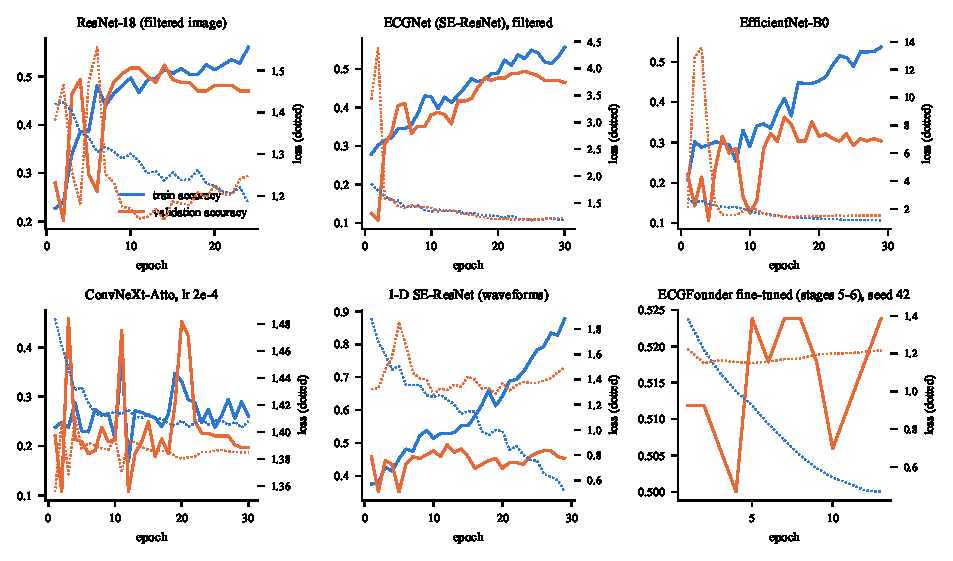
\includegraphics[width=1.00\linewidth,height=0.80\textheight,keepaspectratio]{figures/fig_3_2}
\caption{Training curves of six representative networks: training and validation accuracy (solid) and loss (dotted) per epoch.}\label{fig:3.2}
\end{figure}

\begin{table}[htbp]
\caption{Transfer learning: source, how the knowledge was transferred and what it gave on the hospital printouts.}\label{tab:3.4}
\small
\begin{tabular}{>{\raggedright\arraybackslash\hspace{0pt}}p{\dimexpr 0.199\linewidth-2\tabcolsep\relax}>{\raggedright\arraybackslash\hspace{0pt}}p{\dimexpr 0.295\linewidth-2\tabcolsep\relax}>{\raggedright\arraybackslash\hspace{0pt}}p{\dimexpr 0.505\linewidth-2\tabcolsep\relax}}
\toprule
\textbf{Source} & \textbf{Transfer method} & \textbf{Result on the hospital data} \\
\midrule
ImageNet (1.3 M natural images) & initialise ResNet-18; fine-tune on page images & 0.492 four-class (CV); natural-image features transfer only partly to thin line drawings \\
ECGFounder (10.8 M ECGs, 150 labels) & frozen 1,024-d embedding + linear or MLP head & 0.528--0.542 (CV); screen AUC 0.82; EF $r$ 0.65; best single representation of the project \\
 & partial fine-tuning (stages 5--6; stage 6) & 0.536 (CV); EF $r$ 0.650 against 0.652 frozen: the frozen embedding already holds the EF information \\
 & layer choice (stage 4, 5, 6, diagnostic outputs) & final embedding best (0.544 against 0.517--0.531) \\
EchoNext signals (4,827 US ECG-- echo pairs) & models trained only on EchoNext, applied zero-shot & AUROC 0.85 for EF $\le45$ \%, 0.75 Normal against Mild, EF $ r$ 0.62; four-class 0.551 with no hospital training of the model (only its decision thresholds tuned) \\
 & EchoNext models as stack members & SUPER ensembles 0.583--0.587, the best all-patient results \\
EchoNext images (drawn as printouts) & pre-train pixel CNN, then fine-tune & final ConvNeXt-Tiny ensemble 0.548; ResNet-18: 0.530 against 0.492 with ImageNet only (+3.8 points); EchoNext test accuracy of the pre-trained CNNs 0.58--0.72 \\
\bottomrule
\end{tabular}
\end{table}


Transfer learning was used in four forms, from natural images to EF-labelled ECGs (Table~\ref{tab:3.4}). The closer the source is to the target, the larger the gain: ECG pre-training (ECGFounder) beat ImageNet pre-training by 4--5 points, and EF-labelled public ECGs (EchoNext) supplied the knowledge behind the best ensembles. A model trained only on US patients separates reduced from normal EF on our printouts with AUROC 0.85, which also validates the printout conversion. Frozen ECGFounder features match fine-tuning in EF correlation (0.652 against 0.650) without its over-fitting, and pre-training a pixel CNN on EchoNext ECGs drawn as hospital printouts adds 3.8 points over ImageNet initialisation.

\section{Evaluation protocol}\label{sec:3.6}

\begin{itemize}
  \item \textbf{Cross-validation:} patient-grouped 5-fold CV repeated three times (15 cells), identical folds for every model.
  \item \textbf{Nested choices:} every hyper-parameter, class weight, threshold and ensemble member is chosen inside the training folds \cite{ref37}. Class weights maximise accuracy subject to every recall $\ge0.18$ (fallback 0.15):
\EqThreeThree
  \item \textbf{Intervals and tests:} corrected resampled $t$ statistic \cite{ref38} with Holm adjustment \cite{ref39}:
\EqThreeFour
  \item \textbf{Integrity:} every study was pre-registered in a dated document before it was run; the locked test set was scored once.
\end{itemize}

\chapter{Experimental Study}\label{ch:4}

\begin{table}[htbp]
\caption{Overview of the experimental stages of Phase I.}\label{tab:4.1}
\small
\begin{tabular}{>{\raggedright\arraybackslash\hspace{0pt}}p{\dimexpr 0.151\linewidth-2\tabcolsep\relax}>{\raggedright\arraybackslash\hspace{0pt}}p{\dimexpr 0.319\linewidth-2\tabcolsep\relax}>{\raggedright\arraybackslash\hspace{0pt}}p{\dimexpr 0.212\linewidth-2\tabcolsep\relax}>{\raggedright\arraybackslash\hspace{0pt}}p{\dimexpr 0.315\linewidth-2\tabcolsep\relax}}
\toprule
\textbf{Stage} & \textbf{Main question} & \textbf{Evaluation} & \textbf{Outcome carried forward} \\
\midrule
Original project & Can a page-image CNN grade LVEF? & fixed 210-ECG test set & 27 models; header + ResNet-18 fusion 0.552 \\
Phase 1 & Does a foundation ECG model help? & fixed test set & ECGFounder best for Mild (recall 0.26) \\
Phase 2 & Robust re-evaluation, pre-registered & development CV & ECGFounder MLP fusion 0.544 \\
Phase 3 & Fusion, ensembles, calibration & development CV & vote ensemble C1 0.547 \\
Phase 4 & EF regression, multitask, label quality & development CV & EF $r$ = 0.66; information limit found \\
Phase 5 & Features, boosting, decision rules & development CV & C3 selected, 0.562 \\
Phase 6 / 6A / 6B & Fine-tuning, LSTM family, label variants & development CV & recurrent models tested; C3 kept \\
Label studies & Cleaning, cohorts, abstention & CV and subsets & selective prediction reaches 0.71 \\
Phase 7 & Representations, learning curve, triage & CV, then locked test & triage 0.694 (CV), 0.747 (locked test) \\
Image-only push & HIER, ENH, ULT, EchoNext, SUPER & development CV & ensembles 0.57--0.587 \\
\bottomrule
\end{tabular}
\end{table}


Phase I was carried out in ten stages(Table~\ref{tab:4.1}). Each stage asked one question, and its lesson was carried into the next. Together they produced more than 1,300 recorded results; the Supplementary Tables list every configuration, and Figure~\ref{fig:6.2} in Chapter~\ref{ch:6} compares all model families.

\section{Original project and Phase 1}\label{sec:4.1}

\begin{table}[htbp]
\caption{Representative models of the original project (fixed test set, $n=210$).}\label{tab:4.2}
\small
\begin{tabular}{>{\raggedright\arraybackslash\hspace{0pt}}p{\dimexpr 0.403\linewidth-2\tabcolsep\relax}>{\raggedright\arraybackslash\hspace{0pt}}p{\dimexpr 0.118\linewidth-2\tabcolsep\relax}>{\raggedright\arraybackslash\hspace{0pt}}p{\dimexpr 0.118\linewidth-2\tabcolsep\relax}>{\raggedright\arraybackslash\hspace{0pt}}p{\dimexpr 0.132\linewidth-2\tabcolsep\relax}>{\raggedright\arraybackslash\hspace{0pt}}p{\dimexpr 0.111\linewidth-2\tabcolsep\relax}>{\raggedright\arraybackslash\hspace{0pt}}p{\dimexpr 0.117\linewidth-2\tabcolsep\relax}}
\toprule
\textbf{Model} & \textbf{Accuracy} & \textbf{Bal. acc.} & \textbf{Macro-F1} & \textbf{QWK} & \textbf{HF AUC} \\
\midrule
HOG + PCA + RBF-SVM (classical) & 0.481 & 0.322 & 0.283 & 0.229 & 0.737 \\
ECGNet (custom SE-ResNet) & 0.471 & 0.360 & 0.262 & 0.389 & 0.745 \\
ResNet-18, ImageNet initialised & 0.486 & 0.356 & 0.323 & 0.290 & 0.735 \\
EfficientNet-B0 / MobileNetV3-L (from scratch) & 0.300 / 0.143 & 0.318 / 0.243 & 0.236 / 0.111 & -- & 0.712 / 0.649 \\
1-D ResNet on digitised waveforms ($\times5$ seeds) & 0.457 & 0.364 & 0.358 & 0.410 & 0.752 \\
XGBoost on engineered waveform features & 0.490 & 0.377 & 0.373 & 0.382 & 0.742 \\
Logistic regression on header measurements & 0.514 & 0.442 & 0.421 & 0.422 & 0.795 \\
\textbf{Header 0.6 + ResNet-18 0.4 (default pipeline)} & \textbf{0.552} & 0.454 & 0.433 & 0.447 & 0.791 \\
Always ``Normal'' (reference) & 0.457 & 0.250 & 0.157 & 0 & -- \\
\bottomrule
\end{tabular}
\end{table}


\begin{table}[htbp]
\caption{Phase 1 key models (fixed test set).}\label{tab:4.3}
\small
\begin{tabular}{>{\raggedright\arraybackslash\hspace{0pt}}p{\dimexpr 0.414\linewidth-2\tabcolsep\relax}>{\raggedright\arraybackslash\hspace{0pt}}p{\dimexpr 0.119\linewidth-2\tabcolsep\relax}>{\raggedright\arraybackslash\hspace{0pt}}p{\dimexpr 0.113\linewidth-2\tabcolsep\relax}>{\raggedright\arraybackslash\hspace{0pt}}p{\dimexpr 0.123\linewidth-2\tabcolsep\relax}>{\raggedright\arraybackslash\hspace{0pt}}p{\dimexpr 0.131\linewidth-2\tabcolsep\relax}>{\raggedright\arraybackslash\hspace{0pt}}p{\dimexpr 0.098\linewidth-2\tabcolsep\relax}}
\toprule
\textbf{Model} & \textbf{Accuracy} & \textbf{Bal. acc.} & \textbf{Macro-F1} & \textbf{Mild recall} & \textbf{HF AUC} \\
\midrule
Default pipeline, reproduced & 0.552 & 0.454 & 0.433 & 0.106 & 0.791 \\
A1 ECGFounder, frozen & 0.500 & 0.421 & 0.412 & 0.234 & 0.810 \\
\textbf{A2 ECGFounder, fine-tuned (3-seed ensemble)} & 0.524 & \textbf{0.464} & \textbf{0.448} & \textbf{0.255} & 0.812 \\
A2 with a cumulative-link ordinal head & 0.510 & 0.417 & 0.393 & 0.170 & 0.790 \\
A1 with a CORAL ordinal head & 0.390 & 0.376 & 0.345 & 0.489 & -- \\
Header + A2 fusion & 0.505 & 0.445 & 0.425 & 0.213 & \textbf{0.819} \\
\bottomrule
\end{tabular}
\end{table}


The original project compared 27 models on the fixed 210-ECG test set: classical HOG features with an SVM, CNNs trained from scratch (ECGNet, EfficientNet-B0, MobileNetV3, ConvNeXt-Atto), ImageNet ResNet-18, a 1-D ResNet on digitised waveforms, gradient boosting on 263 engineered features, and the printed header. Every pre-trained model screened heart failure with AUC 0.73--0.80, and the header + ResNet-18 fusion reached 0.552. Phase 1 introduced ECGFounder, which gave the best balanced accuracy (0.464), macro-F1 (0.448), Mild recall (0.255) and screen AUC (0.81--0.82); it became the backbone of later work.

\section{Phases 2--5: robust evaluation, fusion and decision rules}\label{sec:4.2}

\begin{table}[htbp]
\caption{Phase 5, development cross-validation (min recall = lowest per-class recall; admissible if $\ge$ 0.15).}\label{tab:4.4}
\small
\begin{tabular}{>{\raggedright\arraybackslash\hspace{0pt}}p{\dimexpr 0.360\linewidth-2\tabcolsep\relax}>{\raggedright\arraybackslash\hspace{0pt}}p{\dimexpr 0.225\linewidth-2\tabcolsep\relax}>{\raggedright\arraybackslash\hspace{0pt}}p{\dimexpr 0.162\linewidth-2\tabcolsep\relax}>{\raggedright\arraybackslash\hspace{0pt}}p{\dimexpr 0.250\linewidth-2\tabcolsep\relax}}
\toprule
\textbf{Experiment} & \textbf{Accuracy} & \textbf{Min recall} & \textbf{Note} \\
\midrule
E1 MLP + all engineered feature families & 0.554 & 0.164 & admissible \\
E2 LightGBM & 0.544 & 0.184 & admissible \\
E3 stacking, weighted & 0.547 & 0.184 & admissible \\
E4 hierarchical model & 0.567 & 0.067 & Mild recall below floor \\
\textbf{E5 vote + nested prior rule (C3)} & \textbf{0.562} [0.520, 0.603] & 0.177 & \textbf{selected} \\
E6 signal-quality gating & 0.546 & 0.164 & admissible \\
E7 mixup / augmentation & 0.552 / 0.533 & -- & -- \\
\bottomrule
\end{tabular}
\end{table}


Phase 2 moved all modelling to pre-registered, patient-grouped cross-validation on the 837 development ECGs. Phase 3 combined representations; its soft-vote ensemble C1 (0.547) became the reference. Phase 4 added EF regression from the image (MAE 10.4 points, $r=0.66$, AUROC 0.82 for EF $<41$ \%). Phase 5 selected C3, a vote ensemble with a nested class-prior rule (0.562 with all four classes detected), and showed that the most confident half of the ECGs is graded with 0.66--0.68 accuracy, the first evidence for triage.

\section{Phases 6, 6A and 6B: fine-tuning and the LSTM family}\label{sec:4.3}

\begin{table}[htbp]
\caption{LSTM family: architecture, size, cost and results (development CV, original labels).}\label{tab:4.5}
\footnotesize\setlength{\tabcolsep}{4pt}
\begin{tabular}{>{\raggedright\arraybackslash\hspace{0pt}}p{\dimexpr 0.119\linewidth-2\tabcolsep\relax}>{\raggedright\arraybackslash\hspace{0pt}}p{\dimexpr 0.170\linewidth-2\tabcolsep\relax}>{\raggedright\arraybackslash\hspace{0pt}}p{\dimexpr 0.099\linewidth-2\tabcolsep\relax}>{\raggedright\arraybackslash\hspace{0pt}}p{\dimexpr 0.068\linewidth-2\tabcolsep\relax}>{\raggedright\arraybackslash\hspace{0pt}}p{\dimexpr 0.110\linewidth-2\tabcolsep\relax}>{\raggedright\arraybackslash\hspace{0pt}}p{\dimexpr 0.090\linewidth-2\tabcolsep\relax}>{\raggedright\arraybackslash\hspace{0pt}}p{\dimexpr 0.152\linewidth-2\tabcolsep\relax}>{\raggedright\arraybackslash\hspace{0pt}}p{\dimexpr 0.106\linewidth-2\tabcolsep\relax}>{\raggedright\arraybackslash\hspace{0pt}}p{\dimexpr 0.082\linewidth-2\tabcolsep\relax}}
\toprule
\textbf{ID} & \textbf{Input} & \textbf{Layers} & \textbf{Dir.} & \textbf{Params} & \textbf{Train min} & \textbf{Accuracy [95 \% CI]} & \textbf{Macro-F1} & \textbf{HF AUC} \\
\midrule
L0 & rhythm strip (1 ch) & 1 & uni & 17,668 & 0.31 & 0.426 [0.387, 0.466] & 0.257 & 0.570 \\
L1 & aligned (26 ch) & 1 & uni & 24,068 & 0.33 & 0.452 [0.399, 0.504] & 0.324 & 0.697 \\
L2 & aligned & 2 & uni & 57,348 & 0.47 & 0.483 [0.437, 0.529] & 0.352 & 0.714 \\
L3 & aligned & 1 & bi & 48,132 & 0.44 & 0.467 [0.417, 0.516] & 0.337 & 0.704 \\
L4 & aligned & 2 & bi & 147,460 & 0.74 & 0.472 [0.424, 0.519] & 0.339 & 0.718 \\
LSTM-sel & nested choice of L0--L4 & -- & -- & 24k--147k & 2.29 & 0.470 [0.424, 0.515] & 0.344 & 0.721 \\
L5 CNN-LSTM & aligned, 3 conv layers & 1 & bi & 116,580 & 0.38 & 0.484 [0.435, 0.532] & 0.368 & 0.761 \\
\bottomrule
\end{tabular}
\end{table}


\begin{table}[htbp]
\caption{LSTM fusions (development CV, original labels).}\label{tab:4.6}
\small
\begin{tabular}{>{\raggedright\arraybackslash\hspace{0pt}}p{\dimexpr 0.324\linewidth-2\tabcolsep\relax}>{\raggedright\arraybackslash\hspace{0pt}}p{\dimexpr 0.187\linewidth-2\tabcolsep\relax}>{\raggedright\arraybackslash\hspace{0pt}}p{\dimexpr 0.123\linewidth-2\tabcolsep\relax}>{\raggedright\arraybackslash\hspace{0pt}}p{\dimexpr 0.122\linewidth-2\tabcolsep\relax}>{\raggedright\arraybackslash\hspace{0pt}}p{\dimexpr 0.097\linewidth-2\tabcolsep\relax}>{\raggedright\arraybackslash\hspace{0pt}}p{\dimexpr 0.145\linewidth-2\tabcolsep\relax}}
\toprule
\textbf{Model} & \textbf{Accuracy [95 \% CI]} & \textbf{Macro-F1} & \textbf{Mild recall} & \textbf{HF AUC} & \textbf{Params} \\
\midrule
F4 vote + LSTM-sel + prior rule & 0.559 [0.517, 0.600] & 0.449 & 0.182 & 0.834 & C1 + 24k--147k \\
F3 vote + LSTM-sel & 0.553 [0.508, 0.597] & 0.453 & 0.198 & 0.834 & C1 + 24k--147k \\
F2 CNN-LSTM + header + ECGFounder & 0.551 [0.517, 0.585] & 0.452 & 0.166 & 0.834 & 198,820 \\
F1 LSTM + header + ECGFounder & 0.540 [0.507, 0.573] & 0.439 & 0.151 & 0.831 & 130,372 \\
L6 CNN-LSTM + header & 0.497 [0.456, 0.539] & 0.389 & 0.182 & 0.799 & 116,644 \\
\bottomrule
\end{tabular}
\end{table}


\begin{figure}[htbp]
\centering
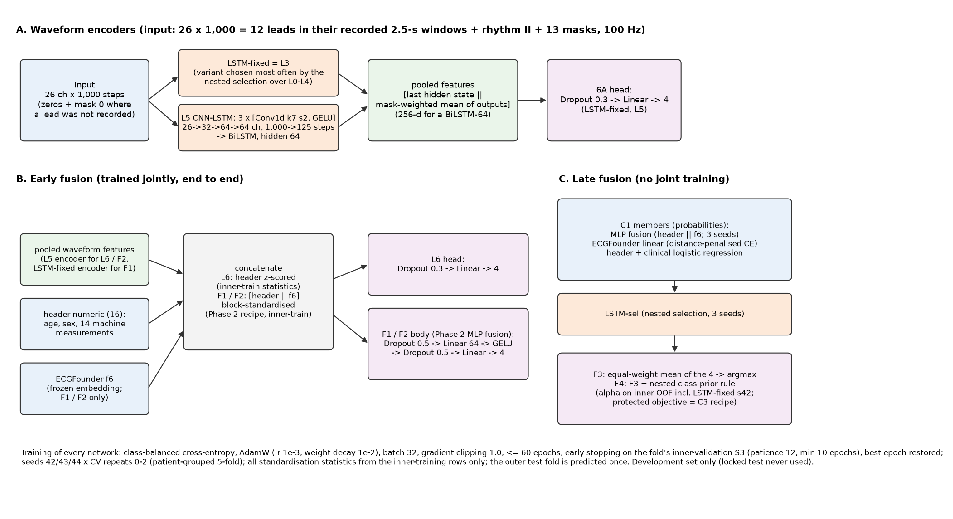
\includegraphics[width=1.00\linewidth,height=0.80\textheight,keepaspectratio]{figures/fig_4_1}
\caption{Phase 6B architectures: waveform encoders (A), early fusion with the header and ECGFounder (B) and late fusion with the vote ensemble (C).}\label{fig:4.1}
\end{figure}

Fine-tuning ECGFounder and adding a second encoder (ECG-FM) did not raise the EF correlation above the frozen embedding ($r\approx0.65$), which confirmed it as the best representation. Phase 6A then built a family of recurrent networks that read the waveform directly (Table~\ref{tab:4.5}): five LSTM variants with 1--2 layers and 64 hidden units, a nested selection among them, and a CNN-LSTM with a three-layer convolutional front-end. The CNN-LSTM had the best screen AUC (0.76) and Mild recall (0.19) of the family with only 117 thousand parameters. Fused with ECGFounder in Phase 6B, the recurrent encoders reached the level of the best ensembles (0.55--0.56, screen AUC 0.83).

\section{Label-quality, cohort and abstention studies}\label{sec:4.4}

Pre-registered studies asked whether cleaner labels, reliable cohorts or abstention could lift performance. On ECGs with clear or verified labels the models score in the 60s and 70s (0.668 on 582 clear-cut ECGs, 0.677 on 620 kept after removing suspect labels, 0.707 on 264 clean, clear-cut ECGs), and selective prediction reaches 0.71 on 22 \% of ECGs. Clinician-style features identified interpretable Mild markers: a spatial QRS--T angle above 100$^{\circ}$ in 52 \% of Mild against 20 \% of Normal ECGs, and poor R-wave progression in 31 \% against 7 \%.

\section{Phase 7 and the image-only ensembles}\label{sec:4.5}

\begin{table}[htbp]
\caption{Label-quality, cohort and abstention studies (development CV).}\label{tab:4.7}
\small
\begin{tabular}{>{\raggedright\arraybackslash\hspace{0pt}}p{\dimexpr 0.404\linewidth-2\tabcolsep\relax}>{\raggedright\arraybackslash\hspace{0pt}}p{\dimexpr 0.303\linewidth-2\tabcolsep\relax}>{\raggedright\arraybackslash\hspace{0pt}}p{\dimexpr 0.291\linewidth-2\tabcolsep\relax}}
\toprule
\textbf{Study} & \textbf{Result} & \textbf{Finding} \\
\midrule
VER: 15 labels corrected to a high-confidence echo & C3 0.565 & label noise costs less than one point \\
HC30: exact-name links within 30 days (395 ECGs) & 0.594; 0.603 with all ECG factors & reliable links give about 0.60 \\
CLEAR: train without 255 border ECGs & 0.668 on the 582 clear-cut ECGs & clear cases are graded well \\
MMCLEAN: remove 217 suspect Mild/Moderate labels & 0.677 on the 620 kept ECGs & accuracy follows label clarity \\
NF / NFS: noise-free training & 0.707 on 264 clean, clear-cut ECGs & strong performance on clean labels \\
MILDFEAT: image-only clinician features & spatial QRS-T angle best single marker & interpretable Mild markers found \\
MILDFIX: Mild-aware, ordinal and EF-based rules & best Mild recall 0.218 at 0.537 & Mild can be traded for accuracy \\
Selective prediction (nested thresholds) & 0.71 on 22 \%, 0.70 on 35 \% answered & confidence is informative \\
\bottomrule
\end{tabular}
\end{table}


\begin{table}[htbp]
\caption{Image-only four-class models (all 837 ECGs, development CV).}\label{tab:4.8}
\small
\begin{tabular}{>{\raggedright\arraybackslash\hspace{0pt}}p{\dimexpr 0.452\linewidth-2\tabcolsep\relax}>{\raggedright\arraybackslash\hspace{0pt}}p{\dimexpr 0.379\linewidth-2\tabcolsep\relax}>{\raggedright\arraybackslash\hspace{0pt}}p{\dimexpr 0.167\linewidth-2\tabcolsep\relax}}
\toprule
\textbf{Model} & \textbf{Accuracy [95 \% CI]} & \textbf{Recall N / Mi / Mo / S} \\
\midrule
HIER: two-stage (Normal / middle / Severe, then Mild vs Moderate) & 0.558 [0.522, 0.594] 0.86 / 0.17 / 0.41 / 0.34 &  \\
HIER-ext (wider tuning grid) & 0.570 [0.527, 0.612] 0.88 / 0.16 / 0.43 / 0.34 &  \\
ENH: synthetic 10-s reconstruction $\rightarrow$ ECGFounder & 0.528 0.76 / 0.18 / 0.44 / 0.41 &  \\
ENH: median-beat shape model & 0.467 0.68 / 0.19 / 0.36 / 0.33 &  \\
ENH: MiniRocket & 0.504 0.74 / 0.22 / 0.38 / 0.33 &  \\
ENH-vote (6 members, tuned class weights) & 0.569 [0.527, 0.610] 0.88 / 0.17 / 0.46 / 0.29 &  \\
\textbf{ULT-stack (10 members + predicted} \textbf{EF)} & \textbf{0.571 [0.542, 0.600]} 0.91 / 0.16 / 0.42 / 0.29 &  \\
ULT2-stack (+ EchoNext-Mini) & 0.569 [0.538, 0.599] 0.90 / 0.15 / 0.44 / 0.28 &  \\
\bottomrule
\end{tabular}
\end{table}


Phase 7 tested new representations and objectives in pilots, measured the learning curve ($+1.4$ accuracy points per doubling of the data) and built header-free cascades. The cascade AGT-img answers only when its EF grade agrees with the image-only classifier and the estimate is far from every class limit: \textbf{0.694 on 56 \%} of ECGs. It was frozen and scored once on the locked test set (\textbf{0.747}). The image-only stacks (HIER, ENH, ULT) then reached 0.570--0.571 without the printed header, above the header-using C3 (0.562).


\chapter{Public-Data Transfer and Image-Only Deep Learning}\label{ch:5}

This chapter adds external knowledge: 4,827 ECG--echocardiography pairs from the public EchoNext data \cite{ref23}, redrawn in the hospital printout format. The EchoNext file was split by patient into 3,853 training and 974 locked EchoNext test ECGs.

\section{EchoNext in the printout format}\label{sec:5.1}

\begin{table}[htbp]
\caption{EchoNext-trained models: internal checks and transfer to the 837 hospital ECGs without any hospital training.}\label{tab:5.1}
\small
\begin{tabular}{>{\raggedright\arraybackslash\hspace{0pt}}p{\dimexpr 0.225\linewidth-2\tabcolsep\relax}%
>{\raggedright\arraybackslash\hspace{0pt}}p{\dimexpr 0.090\linewidth-2\tabcolsep\relax}%
>{\raggedright\arraybackslash\hspace{0pt}}p{\dimexpr 0.090\linewidth-2\tabcolsep\relax}%
>{\raggedright\arraybackslash\hspace{0pt}}p{\dimexpr 0.125\linewidth-2\tabcolsep\relax}%
>{\raggedright\arraybackslash\hspace{0pt}}p{\dimexpr 0.110\linewidth-2\tabcolsep\relax}%
>{\raggedright\arraybackslash\hspace{0pt}}p{\dimexpr 0.120\linewidth-2\tabcolsep\relax}%
>{\raggedright\arraybackslash\hspace{0pt}}p{\dimexpr 0.100\linewidth-2\tabcolsep\relax}%
>{\raggedright\arraybackslash\hspace{0pt}}p{\dimexpr 0.140\linewidth-2\tabcolsep\relax}}
\toprule
 & \multicolumn{2}{>{\raggedright\arraybackslash\hspace{0pt}}p{\dimexpr 0.180\linewidth-2\tabcolsep\relax}}{\textbf{EchoNext locked test (974)}}
 & \multicolumn{4}{>{\raggedright\arraybackslash\hspace{0pt}}p{\dimexpr 0.445\linewidth-2\tabcolsep\relax}}{\textbf{Hospital transfer AUROC / $\bm{r}$}}
 & \textbf{Zero-shot} \\
\cmidrule(lr){2-3}\cmidrule(lr){4-7}\cmidrule(lr){8-8}
\textbf{Model} & \textbf{Acc.} & \textbf{EF $\bm{r}$} & \textbf{EF$\bm{\le}$45} & \textbf{N vs Mi} & \textbf{Mi vs Mo} & \textbf{EF $\bm{r}$} & \textbf{4-class acc.} \\
\midrule
EN-cls (plan, ECGFounder embeddings) & 0.586 & 0.603 & 0.835 & 0.755 & 0.619 & 0.616 & 0.513 \\
EN-all, harmonised hospital input & 0.648 & 0.629 & \textbf{0.846} & \textbf{0.768} & 0.615 & \textbf{0.622} & 0.554 \\
EN-all, plain hospital input & -- & -- & 0.836 & 0.760 & 0.609 & 0.620 & \textbf{0.560} \\
\bottomrule
\end{tabular}
\end{table}


EchoNext waveforms were converted back to millivolts, resampled to 500 Hz, harmonised to the hospital baseline and cut into the printout's 2.5-s windows. The converted signals behave like the hospital's: heart-rate agreement $r=0.96$, QRS duration 82 against 82 ms and QTc 415 against 416 ms. Models trained only on EchoNext were then applied to the hospital printouts. \textbf{Transfer result.} Without any hospital training of the model, the EchoNext-trained classifier

separates EF $\le45$ \% from higher EF with AUROC \textbf{0.846}, Normal from Mild with 0.768, and estimates EF with $ r=0.62$. With only its decision thresholds tuned on the hospital training folds it reaches 0.551 four-class accuracy.

\section{Pruned ensembles of all image-derived models}\label{sec:5.2}

\begin{table}[htbp]
\caption{All ensemble variants (837 ECGs, original labels, corrected 95 \% CI). Members are the mean kept per fold.}\label{tab:5.2}
\footnotesize\setlength{\tabcolsep}{4pt}
\begin{tabular}{>{\raggedright\arraybackslash\hspace{0pt}}p{\dimexpr 0.076\linewidth-2\tabcolsep\relax}>{\raggedright\arraybackslash\hspace{0pt}}p{\dimexpr 0.100\linewidth-2\tabcolsep\relax}>{\raggedright\arraybackslash\hspace{0pt}}p{\dimexpr 0.150\linewidth-2\tabcolsep\relax}>{\raggedright\arraybackslash\hspace{0pt}}p{\dimexpr 0.139\linewidth-2\tabcolsep\relax}>{\raggedright\arraybackslash\hspace{0pt}}p{\dimexpr 0.174\linewidth-2\tabcolsep\relax}>{\raggedright\arraybackslash\hspace{0pt}}p{\dimexpr 0.159\linewidth-2\tabcolsep\relax}>{\raggedright\arraybackslash\hspace{0pt}}p{\dimexpr 0.110\linewidth-2\tabcolsep\relax}>{\raggedright\arraybackslash\hspace{0pt}}p{\dimexpr 0.089\linewidth-2\tabcolsep\relax}}
\toprule
\textbf{Pool} & \textbf{Selection} & \textbf{Meta-learner} & \textbf{Members} & \textbf{Accuracy [95 \% CI]} & \textbf{Recall N / Mi / Mo / S} & \textbf{Macro-F1} & \textbf{Adm.} \\
\midrule
base & greedy & LR (SUPER) & 3.1 & 0.583 [0.540, 0.626] & 0.90 / 0.15 / 0.50 / 0.27 & 0.451 & yes \\
base & greedy & STAGED-4 & 3.1 & 0.581 [0.535, 0.627] & 0.89 / 0.17 / 0.50 / 0.25 & 0.450 & yes \\
base & greedy & ordinal & 3.1 & 0.578 [0.537, 0.620] & 0.89 / 0.17 / 0.49 / 0.28 & 0.450 & yes \\
base & TOP10 & LR & 10 & 0.577 [0.556, 0.598] & 0.88 / 0.15 / 0.52 / 0.26 & 0.447 & yes \\
base & TOP10 & STAGED-4 & 10 & 0.581 [0.555, 0.607] & 0.89 / 0.16 / 0.50 / 0.29 & 0.454 & yes \\
base & TOP10 & \textbf{ordinal} & 10 & \textbf{0.587 [0.565, 0.610]} & 0.89 / 0.17 / \textbf{0.52} / \textbf{0.31} & \textbf{0.467} & yes \\
X & greedy & LR & 3.4 & 0.575 [0.540, 0.611] & 0.89 / 0.16 / 0.48 / 0.25 & 0.442 & yes \\
X & greedy & STAGED-4 & 3.4 & 0.575 [0.541, 0.610] & 0.88 / 0.17 / 0.50 / 0.25 & 0.444 & yes \\
X & greedy & ordinal & 3.4 & 0.577 [0.545, 0.610] & 0.90 / 0.18 / 0.46 / 0.27 & 0.448 & yes \\
X & TOP10 & LR & 10 & 0.579 [0.556, 0.603] & 0.91 / 0.15 / 0.47 / 0.26 & 0.443 & no \\
X & TOP10 & \textbf{STAGED-4} & 10 & \textbf{0.585 [0.557, 0.613]} & 0.89 / \textbf{0.18} / 0.51 / 0.26 & 0.455 & yes \\
X & TOP10 & ordinal & 10 & 0.576 [0.552, 0.600] & 0.89 / 0.16 / 0.49 / 0.27 & 0.449 & yes \\
\midrule
\multicolumn{4}{>{\raggedright\arraybackslash\hspace{0pt}}p{\dimexpr 0.466\linewidth-2\tabcolsep\relax}}{C3 (Phase 5 selected model, reads the printed header)} & 0.562 [0.519, 0.605] & 0.85 / 0.18 / 0.46 / 0.34 & 0.449 & yes \\
\bottomrule
\end{tabular}
\end{table}


Twenty-one image-derived members were pooled: ECGFounder heads, the ENH and ULT members, tabular feature models, the EF band model and the EchoNext-trained models. Inside every training fold, members were selected either greedily (gain $\ge0.002$, at most 10 members) or as the ten best single members (TOP10), and combined by a logistic, staged (STAGED-4: Normal / middle / Severe, then Mild against Moderate) or ordinal (Frank--Hall) meta-learner (Table~\ref{tab:5.2}). The best ensemble, SUPER-TOP10 with the ordinal meta-learner, reaches \textbf{0.587} [0.565, 0.610] with all four classes detected; the staged ensemble reaches \textbf{0.585}.

\section{Additional features for Mild and Moderate}\label{sec:5.3}

Seventy-three further features targeted the Mild and Moderate classes: repolarisation heterogeneity (TCRT, T-wave morphology dispersion, T complexity, non-dipolar residuum), QT dispersion, the QT variability index and per-lead R amplitude ratios. The strongest single markers were TCRT (AUROC 0.738 for Normal against reduced EF) and the lead I R ratio (0.731). They were added as members of the extended ensemble pool (X), which gave the best staged model.

\section{Image-only pixel models with EchoNext pre-training}\label{sec:5.4}

\begin{figure}[htbp]
\centering
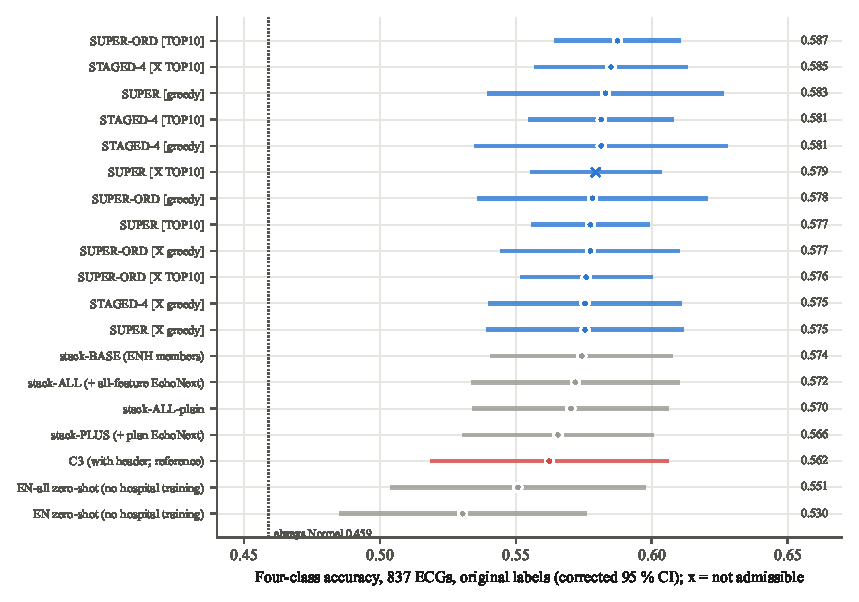
\includegraphics[width=0.91\linewidth,height=0.80\textheight,keepaspectratio]{figures/fig_5_1}
\caption{Four-class accuracy of every stack and ensemble variant of the public-data study, with cor- rected 95 \% confidence intervals.}\label{fig:5.1}
\end{figure}

\begin{table}[htbp]
\caption{Pixel models on the 837 hospital images (class weights tuned inside the training folds).}\label{tab:5.3}
\small
\begin{tabular}{>{\raggedright\arraybackslash\hspace{0pt}}p{\dimexpr 0.298\linewidth-2\tabcolsep\relax}>{\raggedright\arraybackslash\hspace{0pt}}p{\dimexpr 0.142\linewidth-2\tabcolsep\relax}>{\raggedright\arraybackslash\hspace{0pt}}p{\dimexpr 0.157\linewidth-2\tabcolsep\relax}>{\raggedright\arraybackslash\hspace{0pt}}p{\dimexpr 0.167\linewidth-2\tabcolsep\relax}>{\raggedright\arraybackslash\hspace{0pt}}p{\dimexpr 0.123\linewidth-2\tabcolsep\relax}>{\raggedright\arraybackslash\hspace{0pt}}p{\dimexpr 0.110\linewidth-2\tabcolsep\relax}}
\toprule
\textbf{Model} & \textbf{Accuracy [95 \% CI]} & \textbf{Recall N / Mi / Mo / S} & \textbf{Precision N / Mi / Mo / S} & \textbf{Macro-F1} & \textbf{Inner-val acc.} \\
\midrule
FT-IN: ResNet-18, ImageNet only & 0.492 [0.446, 0.537] & 0.75 / 0.20 / 0.36 / 0.24 & 0.69 / 0.23 / 0.37 / 0.25 & 0.386 & -- \\
ZS: ResNet-18, EchoNext only & 0.524 [0.493, 0.556] & 0.86 / 0.18 / 0.27 / 0.32 & 0.63 / 0.27 / 0.42 / 0.37 & 0.403 & -- \\
FT-EN: ResNet-18, EchoNext + fine-tuning & 0.530 [0.481, 0.578] & 0.82 / \textbf{0.23} / 0.34 / 0.29 & 0.71 / 0.29 / 0.38 / 0.29 & 0.416 & 0.569 \\
E2: ConvNeXt-T 384 $\times$ 768 & 0.535 [0.484, 0.586] & 0.80 / 0.22 / 0.40 / 0.31 & -- & \textbf{0.433} & 0.583 \\
E3: ConvNeXt-T, EF-led + EF grading & 0.540 [0.511, 0.570] & 0.86 / 0.17 / 0.35 / 0.34 & -- & 0.419 & 0.597 \\
E4: E3 + layer-wise LR, mixup, TTA, 3 seeds (final) & \textbf{0.548 [0.513, 0.582]} & 0.85 / 0.18 / 0.41 / 0.28 & -- & 0.423 & \textbf{0.604} \\
E6: triage on E4 (answers 60.6 \%) & 0.661 on answered & -- & -- & -- & -- \\
E5: stack-ALL + E3 network (pixels + traces) & 0.569 [0.534, 0.604] & 0.90 / 0.17 / 0.42 / 0.26 & -- & -- & -- \\
\bottomrule
\end{tabular}
\end{table}


Pixel CNNs read the page image directly. EchoNext ECGs were drawn as hospital printouts and used to pre-train them, before fine-tuning on the hospital images. Pre-training on the printoutformat EchoNext images raised ResNet-18 from 0.492 (ImageNet only) to 0.530. The final model, a three-seed ConvNeXt-Tiny ensemble trained with an EF-led loss, layer-wise learning rates, mixup and test-time augmentation, reached \textbf{0.548} [0.513, 0.582] from the page pixels alone (Table~\ref{tab:5.3}), within about two points of C3, which also reads the printed measurements. As a triage model it answers 60.6 \% of the ECGs at 0.661, and its 50 \% most confident ECGs are graded with 0.70 accuracy (descriptive). Added to the stacks, the pixel network gave 0.569.


\chapter{Results and Discussion}\label{ch:6}

\section{Headline results}\label{sec:6.1}

\begin{table}[htbp]
\caption{Headline results of Phase I (image-derived inputs only; original four-class labels).}\label{tab:6.1}
\small
\begin{tabular}{>{\raggedright\arraybackslash\hspace{0pt}}p{\dimexpr 0.200\linewidth-2\tabcolsep\relax}>{\raggedright\arraybackslash\hspace{0pt}}p{\dimexpr 0.321\linewidth-2\tabcolsep\relax}>{\raggedright\arraybackslash\hspace{0pt}}p{\dimexpr 0.210\linewidth-2\tabcolsep\relax}>{\raggedright\arraybackslash\hspace{0pt}}p{\dimexpr 0.267\linewidth-2\tabcolsep\relax}}
\toprule
\textbf{Result} & \textbf{Model} & \textbf{Accuracy [95 \% CI]} & \textbf{Population} \\
\midrule
\textbf{Best on all patients} & Ten-member ensemble with ordinal meta-learner (SUPER-TOP10-ORD) & \textbf{0.587} [0.565, 0.610] & all 837 development ECGs (cross-validation) \\
Best staged model & STAGED-4 on the extended pool & 0.585 [0.557, 0.613] & all 837 development ECGs \\
\textbf{Best in the 60s} & Image-only triage model & \textbf{0.694} [0.655, 0.736] & the 56 \% of patients it answers (cross-validation) \\
\textbf{Best in the 70s} & Same frozen triage model, scored once & \textbf{0.747} [0.660, 0.837] & the 50 \% of unseen locked-test patients it answers \\
\bottomrule
\end{tabular}
\end{table}


Three results summarise Phase I. Each is the strongest of its kind, and each was obtained under the full protocol of Section~\ref{sec:3.6}.

\subsection{Best on all patients: 0.587}\label{sec:6.1.1}

The ensemble keeps, inside every training fold, the ten best of 21 image-derived members. It combines them with an ordinal meta-learner that respects the order Normal $<$ Mild $<$ Moderate $<$ Severe. Why this result is strong:

\begin{itemize}
  \item \textbf{Close to the achievable limit.} At the EF precision of the best ECG-based estimators (error SD about 13 points), the simulation of Section~\ref{sec:6.5} predicts 0.592 four-class accuracy for a perfect grader. The ensemble reaches 0.587, about 99 \% of that level.
  \item \textbf{Better without the printed numbers.} It exceeds the Phase 5 selected model C3, which also reads the machine measurements printed on the page (0.562). It also exceeds the original project's page-image CNN (0.471) by 11.6 points.
  \item \textbf{Every class detected.} Normal recall is 0.89, Mild 0.17, Moderate 0.52 and Severe 0.31. Moderate recall rose from 0.42 (stack-BASE) to 0.52, and macro-F1 is the highest of the project (0.467).
  \item \textbf{Stable.} The 95 \% interval is only $\pm0.022$ wide, half that of earlier ensembles. The three repeats agree closely (0.580, 0.597, 0.585).
  \item \textbf{Robust to the choice of combiner.} The pre-declared greedy ensemble (0.583) and the staged ensemble (0.585) land within 0.004 of it, so the result does not depend on one particular combiner.
  \item \textbf{Uses public knowledge.} EchoNext-trained members are selected in most folds, including the EchoNext LightGBM and the pixel network's EF band. The ensemble therefore draws on information learned from thousands of external patients.
\end{itemize}
\subsection{Best in the 60s: 0.694 on the answered patients}\label{sec:6.1.2}

The triage model estimates EF from the image and grades it. It gives a four-class answer only when two conditions hold:

\begin{itemize}
  \item the EF grade agrees with the image-only four-class classifier;
  \item the estimate is at least 3.05 EF points from every class limit.
\end{itemize}
Otherwise it recommends echocardiography. Why this result is strong:

\begin{enumerate}
  \item \textbf{Built without seeing the test data.} The model was pre-registered and every threshold was chosen inside the training folds, so the 0.694 is an honest out-of-sample estimate.
  \item \textbf{A large margin over the all-patient task.} The lower confidence bound (0.655) is above the best all-patient accuracy (0.587). The gain on the answered patients is therefore not noise.
  \item \textbf{Grounded in the physics of the problem.} Errors concentrate at the class limits. ECGs whose echo EF is at least 10 points from every limit are classified with 79--84 \% accuracy, while those within 6 points are mostly wrong(Figure~\ref{fig:6.8}). The margin rule turns this observation into a decision rule.
  \item \textbf{Two independent views must agree.} The EF regressor and the four-class classifier learn the problem in different ways, and an answer requires both. This is a natural safeguard against isolated errors.
  \item \textbf{Calibrated confidence.} Across the project, accuracy rises steadily as fewer, more confident cases are answered (Figure~\ref{fig:6.5}):
\end{enumerate}
\begin{itemize}
  \item about 0.66--0.68 on the most confident 50 \% (Phase 5);
  \item 0.694 on 56 \% (triage);
  \item about 0.71 on 22 \% (selective prediction).
\end{itemize}
\begin{enumerate}
  \item \textbf{Clinically meaningful answers.} 90 \% [86, 94] of its confident ``Normal'' answers have an echo EF of at least 41 \%, which rules out moderate or severe dysfunction for these patients.
  \item \textbf{Halves the workload.} It gives a confident answer for more than half of the patients, which could roughly halve the number of echocardiograms needed for triage in a screening setting.
  \item \textbf{Image only.} It uses only the ECG printout, the document every hospital already has.
\end{enumerate}
\subsection{Best in the 70s: 0.747 on unseen patients}\label{sec:6.1.3}

The same model was frozen (its file recorded by a SHA-256 hash) and then scored once on the 210-ECG locked test set. Why this result is strong:

\begin{enumerate}
  \item \textbf{Truly unseen patients.} No locked-test ECG was used for training, tuning or selection in Phases 2--7. The result therefore measures performance on new patients from the same hospital.
  \item \textbf{Better than its own estimate.} The locked-test accuracy (0.747) is above the cross-validation estimate (0.694). Every development estimate lies inside its locked-test interval (Figure~\ref{fig:6.1}), so the model does not overfit the development data.
  \item \textbf{Stable answered share.} The model answered 49.7 \% [42.9, 56.7] of the test patients, against 56 \% in cross-validation. Its confidence behaves the same on new data.
  \item \textbf{Four-class performance carries over.} The underlying image-only classifier reached 0.553 [0.485, 0.621] on the test set, against 0.558 in cross-validation. Its Mild precision and recall were 0.32 and 0.32.
  \item \textbf{Safe confident ``Normal'' answers.} 85 \% [77, 92] of them have EF of at least 41 \%.
  \item \textbf{Robust to the analysis set.} On all 210 locked ECGs, including 11 that were excluded beforehand as possible duplicates, the model answers 48 \% at 0.743.
  \item \textbf{Proper interval.} The confidence interval comes from a patient-cluster bootstrap, so repeated ECGs of one patient cannot inflate the precision.
\end{enumerate}
\section{All models compared}\label{sec:6.2}

\begin{figure}[htbp]
\centering
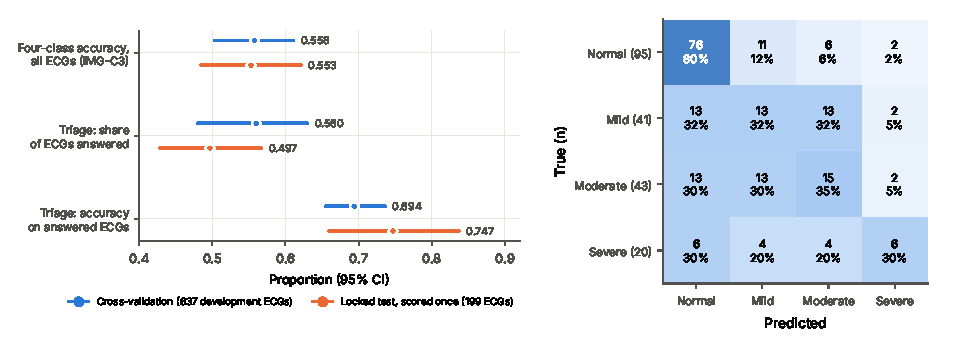
\includegraphics[width=1.00\linewidth,height=0.80\textheight,keepaspectratio]{figures/fig_6_1}
\caption{Left: development estimates and locked-test results of the final model (every cross-validation value lies inside its locked-test interval). Right: locked-test confusion matrix of the four-class image-only classifier.}\label{fig:6.1}
\end{figure}

Figure~\ref{fig:6.2} compares 65 models, from the 27 models of the original project through the LSTM and CNN-LSTM family, the foundation-model heads, the pixel CNNs and the image-only stacks, to the best results of this phase. It is sorted by accuracy, from the locked-test triage result (0.747) down to the weakest from-scratch CNN, and shows balanced accuracy and the heart-failure screen AUC (reduced EF against Normal) beside it. The final ensembles lead on every metric: accuracy 0.583--0.587 and screen AUC 0.844--0.846, against 0.552 and 0.80 for the best original model and 0.43--0.48 and 0.57--0.76 for the stand-alone recurrent models. Figure~\ref{fig:6.3} sorts the same models by screen AUC. Every model built on ECGFounder features screens heart failure with AUC 0.82--0.85, so the foundation-model representation carries most of the signal.

\section{All results in the upper 50s, 60s and 70s}\label{sec:6.3}

Phase I produced 501 configurations with accuracy 0.55 or more: 270 between 0.55 and 0.60 and 231 at 0.60 or above (Figure~\ref{fig:6.4}; all are listed in the Supplementary Tables).

\begin{itemize}
  \item \textbf{All patients (128 results, 0.55--0.587).} Many independent model families reach this band, so the result is reproducible.
  \item \textbf{Answered ECGs (111 results, up to 0.75).} Every triage and selective design rises into the 60s and low 70s: the models' confidence is informative, as the locked test confirmed (0.747).
  \item \textbf{Clean or verified labels (143 results, up to 0.72).} Where the labels are reliable, the same models score in the 60s and 70s.
  \item \textbf{Other definitions (110 results).} The clinically pre-specified ESC 2021 limits give 0.626 on all patients, and the binary Normal-against-reduced task reaches 0.775.
\end{itemize}
\section{Trade-off analysis}\label{sec:6.4}

\begin{figure}[htbp]
\centering
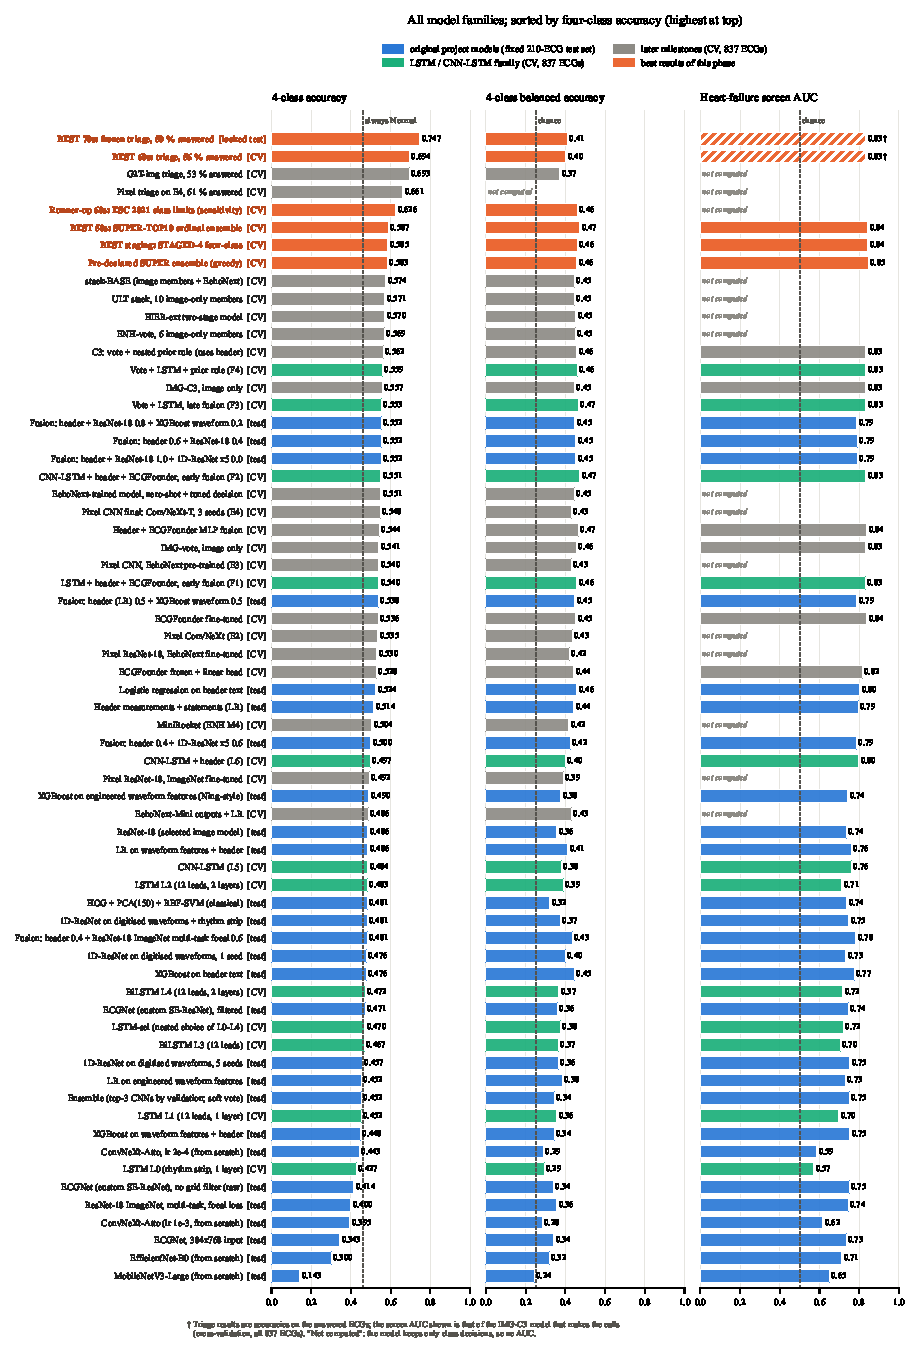
\includegraphics[width=0.97\linewidth,height=0.80\textheight,keepaspectratio]{figures/fig_6_2}
\caption{All model families sorted by four-class accuracy (highest at the top). [test] = fixed 210-ECG test set of the original project; [CV] = cross-validation on 837 development ECGs; [locked test] = frozen model scored once.}\label{fig:6.2}
\end{figure}

\begin{figure}[htbp]
\centering
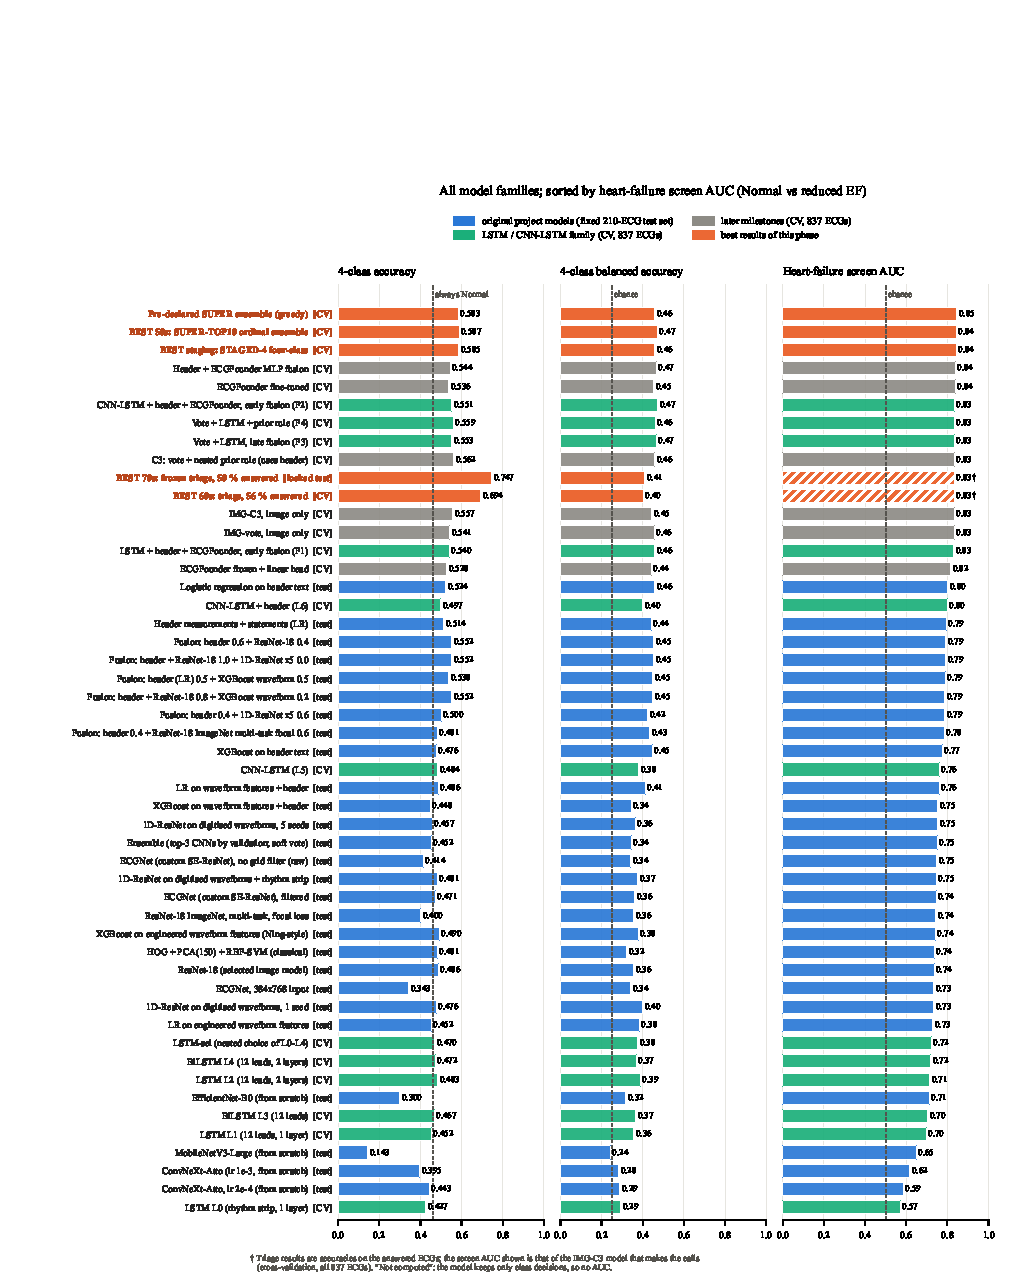
\includegraphics[width=1.00\linewidth,height=0.80\textheight,keepaspectratio]{figures/fig_6_3}
\caption{The same models sorted by heart-failure screen AUC (reduced EF against Normal).}\label{fig:6.3}
\end{figure}

\begin{figure}[htbp]
\centering
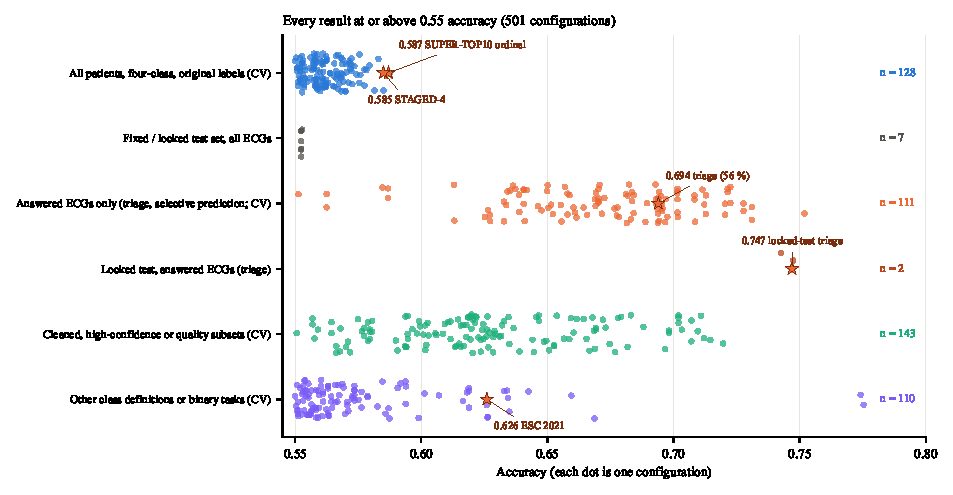
\includegraphics[width=1.00\linewidth,height=0.80\textheight,keepaspectratio]{figures/fig_6_4}
\caption{Every result with accuracy $\ge0.55$, grouped by evaluation population (each dot is one config- uration; stars mark the headline results).}\label{fig:6.4}
\end{figure}

\begin{figure}[htbp]
\centering
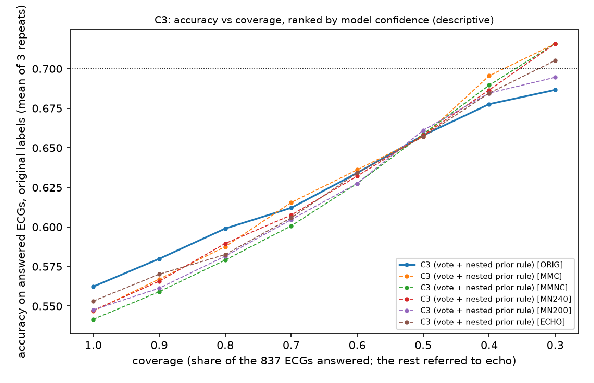
\includegraphics[width=0.63\linewidth,height=0.80\textheight,keepaspectratio]{figures/fig_6_5}
\caption{Accuracy against the share of ECGs answered (selective prediction, nested thresholds).}\label{fig:6.5}
\end{figure}

\textbf{Coverage against accuracy.} Answering fewer, more confident patients raises accuracy steadily (Figure~\ref{fig:6.5}) : the triage model sits at 56 \% coverage and 0.694, and selective prediction reaches about 0.71 at 22 \% coverage.

\textbf{Mild detected against accuracy.} Figure~\ref{fig:6.6} plots accuracy against Mild recall for more than 500 models. Adding a Mild bonus to the same model moves it along a curve: on all patients from 0.56 at Mild recall 0.05 to 0.27 at 0.89. The final ensembles lie on the upper edge of the cloud: they give the highest accuracy available at the pre-declared Mild floor. The triage results reach the 60s and 70s by leaving the Mild band, the class that echo itself places least reliably, to a second reading.

\begin{figure}[htbp]
\centering
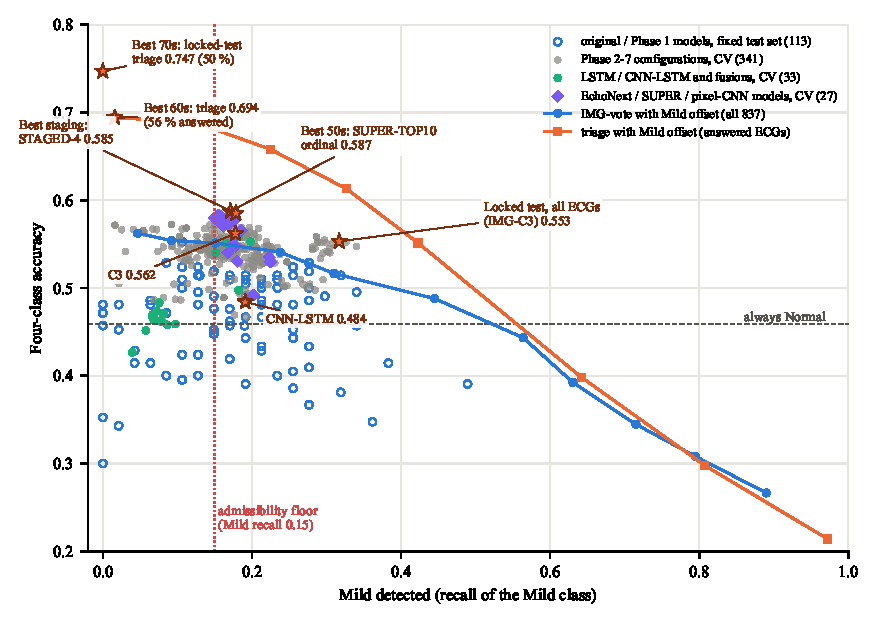
\includegraphics[width=0.93\linewidth,height=0.80\textheight,keepaspectratio]{figures/fig_6_6}
\caption{Mild detected (recall of the Mild class) against four-class accuracy for all models. Stars mark the headline results; lines show the effect of a Mild offset on IMG-vote (all ECGs) and on the triage model (answered ECGs).}\label{fig:6.6}
\end{figure}

\textbf{Class definition.} Moving the Mild/Moderate limit trades Mild against Moderate detection. Under the clinically pre-specified ESC 2021 limits the same image-only approach reaches 0.626 [0.588, 0.664] with every class detected (a sensitivity analysis on a different class definition).

\section{Why the results are strong and why higher accuracy is not fea- sible}\label{sec:6.5}

Every model family, label-cleaning scheme and class definition lands within a few points of the same level. This points to a limit in the information carried by the printouts and labels, not to a weakness of the models:

\begin{itemize}
  \item \textbf{EF precision against band width.} The best ECG-based EF estimators err with SD $\approx13$ points ($ r\approx0.66$), which for these class bands gives 0.592 for a perfect grader; our best model reaches 0.587. Seventy per cent would need SD $\le7.7$, i.e. $ r\approx0.90$, beyond any published AI-ECG model (Figure~\ref{fig:6.7}).
  \item \textbf{Errors sit at the class limits.} 51 \% of the ECGs have an echo EF within 6 points of a limit and are misclassified 62--68 \% of the time, while ECGs at least 10 points from every limit are graded with 79--84 \% accuracy(Figure~\ref{fig:6.8}).
  \item \textbf{The ECG separates extremes, not neighbours.} Pairwise AUROCs are 0.90 for Normal against Severe and 0.88 against Moderate, but 0.75--0.79 for Normal against Mild and 0.62--0.64 for Mild against Moderate.
  \item \textbf{Label consistency.} 6.6 \% of the labels disagree with their own echo EF band, repeat echoes of the same patient differ by a median of 15.4 points, and ECG--echo agreement falls from $r=0.75$ for close links to 0.42 for links more than 30 days apart.
\end{itemize}
\begin{figure}[htbp]
\centering
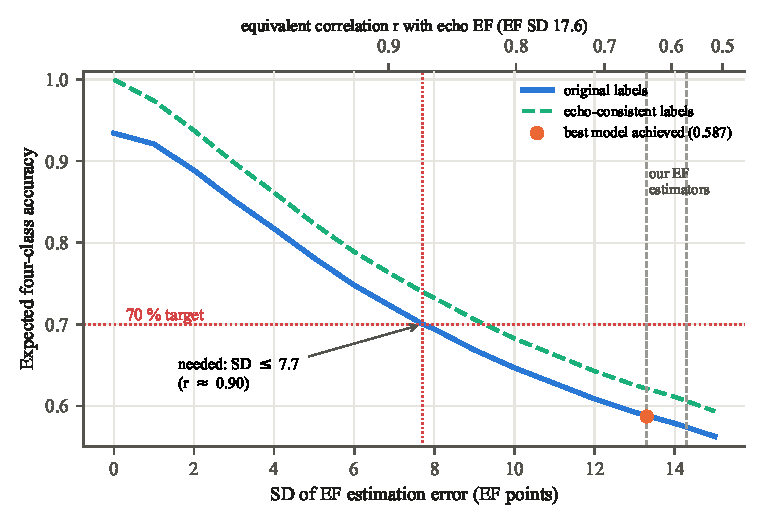
\includegraphics[width=0.76\linewidth,height=0.80\textheight,keepaspectratio]{figures/fig_6_7}
\caption{Expected four-class accuracy against the SD of the EF estimation error (simulation on the 837 development ECGs). Our EF estimators lie at SD 13--14, where the best model (0.587) sits on the curve. 70 \% needs SD $\le7.7$, i.e. $ r\approx0.90$.}\label{fig:6.7}
\end{figure}

\begin{figure}[htbp]
\centering
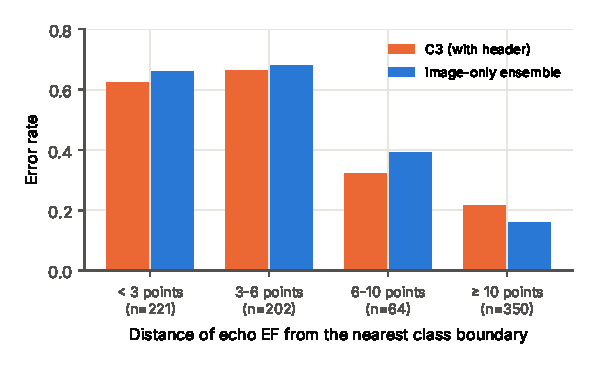
\includegraphics[width=0.58\linewidth,height=0.80\textheight,keepaspectratio]{figures/fig_6_8}
\caption{Error rate by distance of the echo EF from the nearest class limit.}\label{fig:6.8}
\end{figure}

\begin{itemize}
  \item \textbf{Input format and size.} A printout shows each lead for only 2.5 s, and each doubling of the 837 training ECGs adds only about 1.4 points.
\end{itemize}
Exceeding 0.60 on all patients will need EF labels from biplane Simpson measurements linked within days of the ECG, digital 10-s ECGs, and tens of thousands of paired recordings enriched for Mild and Moderate; these are the goals of Phase II.


\chapter{Summary and Conclusions}\label{ch:7}

\section{Conclusions}\label{sec:7.1}

\begin{enumerate}
  \item \textbf{Best on all patients: 0.587} [0.565, 0.610] from image-derived inputs only, about 99 \% of the 0.592 that the EF information of the ECG permits, and above the model that also reads the printed measurements (0.562).
  \item \textbf{Best in the 60s: 0.694} [0.655, 0.736] on the 56 \% of patients the triage model answers in cross-validation.
  \item \textbf{Best in the 70s: 0.747} [0.660, 0.837] on the 50 \% of unseen locked-test patients it answers, above its own development estimate.
  \item \textbf{Transfer works across populations:} a model trained only on US public data detects EF $\le45$ \% on our printouts with AUROC 0.85.
  \item \textbf{The ceiling is set by the labels and the information in the ECG:} 70 \% on all patients would need EF estimates correlating at $r\approx0.90$ with echo, against about 0.66 achievable today.
\end{enumerate}
\section{Scope for future work (Phase II)}\label{sec:7.2}

\begin{itemize}
  \item Larger, multi-year data with biplane-Simpson EF linked by patient identifier within days of the ECG.
  \item Digital 10-s simultaneous ECGs where available, and enrichment for Mild and Moderate patients.
  \item Prospective evaluation of the triage model as an echocardiography-referral aid, and deployment as a lightweight application.
\end{itemize}


% ---------------------------------------------------------------- references (IEEE numbering, as in the template)
\renewcommand{\bibname}{References}
\begingroup
\setstretch{\refstretch}            % template: references at 12 pt, 1.1 line stretch, 9 pt between entries
\chapter*{References}
\phantomsection\addcontentsline{toc}{chapter}{References}
\markboth{References}{}
\renewcommand{\chapter}[2]{}        % thebibliography must not open a second heading
\begin{thebibliography}{99}

\bibitem{ref1} T. A. McDonagh, M. Metra, M. Adamo, R. S. Gardner, A. Baumbach, M. B\"ohm, H. Burri, J. Butler, J. Čelutkienė, O. Chioncel \emph{et al.}, ``2021 ESC Guidelines for the diagnosis and treatment of acute and chronic heart failure,'' \emph{European Heart Journal}, vol. 42, no. 36, pp. 3599--3726, 2021.

\bibitem{ref2} P. A. Heidenreich, B. Bozkurt, D. Aguilar, L. A. Allen, J. J. Byun, M. M. Colvin, A. Deswal, M. H. Drazner, S. M. Dunlay, L. R. Evers \emph{et al.}, ``2022 AHA/ACC/HFSA Guideline for the Management of Heart Failure: A Report of the American College of Cardiology/American Heart Association Joint Committee on Clinical Practice Guidelines,'' \emph{Circulation}, vol. 145, no. 18, pp. e895--e1032, 2022.

\bibitem{ref3} Z. I. Attia, S. Kapa, F. Lopez-Jimenez, P. M. McKie, D. J. Ladewig, G. Satam, P. A. Pellikka, M. Enriquez-Sarano, P. A. Noseworthy, T. M. Munger \emph{et al.}, ``Screening for cardiac contractile dysfunction using an artificial intelligence--enabled electrocardiogram,'' \emph{Nature Medicine}, vol. 25, no. 1, pp. 70--74, 2019.

\bibitem{ref4} X. Yao, D. R. Rushlow, J. W. Inselman, R. G. McCoy, T. D. Thacher, E. M. Behnken, M. E. Bernard, S. L. Rosas, A. Akfaly, A. Misra \emph{et al.}, ``Artificial intelligence--enabled electrocardiograms for identification of patients with low ejection fraction: a pragmatic, randomized clinical trial,'' \emph{Nature} \emph{Medicine}, vol. 27, no. 5, pp. 815--819, 2021.

\bibitem{ref5} R. M. Lang, L. P. Badano, V. Mor-Avi, J. Afilalo, A. Armstrong, L. Ernande, F. A. Flachskampf, E. Foster, S. A. Goldstein, T. Kuznetsova \emph{et al.}, ``Recommendations for Cardiac Chamber Quantification by Echocardiography in Adults: An Update from the American Society of Echocardiography and the European Association of Cardiovascular Imaging,'' \emph{Journal of the American Society of} \emph{Echocardiography}, vol. 28, no. 1, pp. 1--39.e14, 2015.

\bibitem{ref6} P. Thavendiranathan, A. D. Grant, T. Negishi, J. C. Plana, Z. B. Popović, and T. H. Marwick, ``Reproducibility of Echocardiographic Techniques for Sequential Assessment of Left Ventricular Ejection Fraction and Volumes: Application to Patients Undergoing Cancer Chemotherapy,'' \emph{Journal of the} \emph{American College of Cardiology}, vol. 61, no. 1, pp. 77--84, 2013.

\bibitem{ref7} D. G. Strauss, R. H. Selvester, and G. S. Wagner, ``Defining Left Bundle Branch Block in the Era of Cardiac Resynchronization Therapy,'' \emph{The American Journal of Cardiology}, vol. 107, no. 6, pp. 927--934, 2011.

\bibitem{ref8} M. K. Das, B. Khan, S. Jacob, A. Kumar, and J. Mahenthiran, ``Significance of a Fragmented QRS Complex Versus a Q Wave in Patients With Coronary Artery Disease,'' \emph{Circulation}, vol. 113, no. 21, pp. 2495--2501, 2006.

\bibitem{ref9} I. Kardys, J. A. Kors, I. M. van der Meer, A. Hofman, D. A. M. van der Kuip, and J. C. M. Witteman, ``Spatial QRS-T angle predicts cardiac death in a general population,'' \emph{European Heart Journal}, vol. 24, no. 14, pp. 1357--1364, 2003.

\bibitem{ref10} B. Acar, G. Yi, K. Hnatkova, and M. Malik, ``Spatial, temporal and wavefront direction characteristics of 12-lead T-wave morphology,'' \emph{Medical \& Biological Engineering \& Computing}, vol. 37, no. 5, pp. 574--584, 1999.

\bibitem{ref11} R. D. Berger, E. K. Kasper, K. L. Baughman, E. Marban, H. Calkins, and G. F. Tomaselli, ``Beatto-Beat QT Interval Variability: Novel Evidence for Repolarization Lability in Ischemic and Nonischemic Dilated Cardiomyopathy,'' \emph{Circulation}, vol. 96, no. 5, pp. 1557--1565, 1997.

\bibitem{ref12} A. Vaid, K. W. Johnson, M. A. Badgeley, S. S. Somani, M. Bicak, I. Landi, A. Russak, S. Zhao, M. A. Levin, R. S. Freeman \emph{et al.}, ``Using Deep-Learning Algorithms to Simultaneously Identify Right and Left Ventricular Dysfunction From the Electrocardiogram,'' \emph{JACC: Cardiovascular Imaging}, vol. 15, no. 3, pp. 395--410, 2022.

\bibitem{ref13} V. Sangha, A. A. Nargesi, L. S. Dhingra, A. Khunte, B. J. Mortazavi, A. H. Ribeiro, E. Banina, O. Adeola, N. Garg, C. A. Brandt \emph{et al.}, ``Detection of Left Ventricular Systolic Dysfunction From Electrocardiographic Images,'' \emph{Circulation}, vol. 148, no. 9, pp. 765--777, 2023.

\bibitem{ref14} K. K. Shivashankara, Deepanshi, A. Mehri Shervedani, G. D. Clifford, M. A. Reyna, and R. Sameni, ``ECG-Image-Kit: a synthetic image generation toolbox to facilitate deep learning-based electrocardiogram digitization,'' \emph{Physiological Measurement}, vol. 45, no. 5, p. 055019, 2024.

\bibitem{ref15} H. Wu, K. H. K. Patel, X. Li, B. Zhang, C. Galazis, N. Bajaj, A. Sau, X. Shi, L. Sun, Y. Tao \emph{et al.}, ``A fully-automated paper ECG digitisation algorithm using deep learning,'' \emph{Scientific Reports}, vol. 12, no. 1, p. 20963, 2022.

\bibitem{ref16} M. A. Reyna, Deepanshi, J. T. Weigle, Z. Koscova, K. S. Campbell, S. Seyedi, A. Elola, A. Bahrami Rad, A. J. Shah, N. K. Bhatia \emph{et al.}, ``Digitization and Classification of ECG Images: The George B. Moody PhysioNet Challenge 2024,'' in \emph{Computing in Cardiology (CinC 2024)}, vol. 51, 2024.

\bibitem{ref17} A. E. Ulloa-Cerna, L. Jing, J. M. Pfeifer, S. Raghunath, J. A. Ruhl, D. B. Rocha, J. B. Leader, N. Zimmerman, G. Lee, S. R. Steinhubl \emph{et al.}, ``rECHOmmend: An ECG-Based Machine Learning Approach for Identifying Patients at Increased Risk of Undiagnosed Structural Heart Disease Detectable by Echocardiography,'' \emph{Circulation}, vol. 146, no. 1, pp. 36--47, 2022.

\bibitem{ref18} Z. I. Attia, D. M. Harmon, J. Dugan, L. Manka, F. Lopez-Jimenez, A. Lerman, K. C. Siontis, P. A. Noseworthy, X. Yao, E. W. Klavetter \emph{et al.}, ``Prospective evaluation of smartwatch-enabled detection of left ventricular dysfunction,'' \emph{Nature Medicine}, vol. 28, no. 12, pp. 2497--2503, 2022.

\bibitem{ref19} P. Bachtiger, C. F. Petri, F. E. Scott, S. Ri Park, M. A. Kelshiker, H. K. Sahemey, B. Dumea, R. Alquero, P. S. Padam, I. R. Hatrick \emph{et al.}, ``Point-of-care screening for heart failure with reduced ejection fraction using artificial intelligence during ECG-enabled stethoscope examination in London, UK: a prospective, observational, multicentre study,'' \emph{The Lancet Digital Health}, vol. 4, no. 2, pp. e117--e125, 2022.

\bibitem{ref20} A. Khunte, V. Sangha, E. K. Oikonomou, L. S. Dhingra, A. Aminorroaya, B. J. Mortazavi, A. Coppi, C. A. Brandt, H. M. Krumholz, and R. Khera, ``Detection of left ventricular systolic dysfunction from single-lead electrocardiography adapted for portable and wearable devices,'' \emph{npj Digital} \emph{Medicine}, vol. 6, no. 1, p. 124, 2023.

\bibitem{ref21} J. Li, A. D. Aguirre, V. Moura, J. Jin, C. Liu, L. Zhong, C. Sun, G. Clifford, M. B. Westover, and S. Hong, ``An Electrocardiogram Foundation Model Built on over 10 Million Recordings,'' \emph{NEJM} \emph{AI}, vol. 2, no. 7, p. AIoa2401033, 2025.

\bibitem{ref22} K. McKeen, S. Masood, A. Toma, B. Rubin, and B. Wang, ``ECG-FM: an open electrocardiogram foundation model,'' \emph{JAMIA Open}, vol. 8, no. 5, p. ooaf122, 2025.

\bibitem{ref23} T. J. Poterucha, L. Jing, R. P. Ricart, M. Adjei-Mosi, J. Finer, D. Hartzel, C. Kelsey, A. Long, D. Rocha, J. A. Ruhl \emph{et al.}, ``Detecting structural heart disease from electrocardiograms using AI,'' \emph{Nature}, vol. 644, no. 8075, pp. 221--230, 2025.

\bibitem{ref24} J. W. Hughes, L. Jing, J. Finer, D. Hartzel, C. Kelsey, A. Long, D. Rocha, J. Ruhl, T. Poterucha, and P. Elias, ``EchoNext-Mini: A Dataset and Baseline AI Model for Detecting Structural Heart Disease from Electrocardiograms,'' \emph{NEJM AI}, vol. 3, no. 5, p. AIdbp2500516, 2026.

\bibitem{ref25} A. Y. Hannun, P. Rajpurkar, M. Haghpanahi, G. H. Tison, C. Bourn, M. P. Turakhia, and A. Y. Ng, ``Cardiologist-level arrhythmia detection and classification in ambulatory electrocardiograms using a deep neural network,'' \emph{Nature Medicine}, vol. 25, no. 1, pp. 65--69, 2019.

\bibitem{ref26} A. H. Ribeiro, M. H. Ribeiro, G. M. M. Paixão, D. M. Oliveira, P. R. Gomes, J. A. Canazart, M. P. S. Ferreira, C. R. Andersson, P. W. Macfarlane, W. Meira \emph{et al.}, ``Automatic diagnosis of the 12-lead ECG using a deep neural network,'' \emph{Nature Communications}, vol. 11, no. 1, p. 1760, 2020.

\bibitem{ref27} K. He, X. Zhang, S. Ren, and J. Sun, ``Deep Residual Learning for Image Recognition,'' in \emph{Pro-} \emph{ceedings of the IEEE Conference on Computer Vision and Pattern Recognition (CVPR)}, 2016, pp. 770--778.

\bibitem{ref28} M. Tan and Q. Le, ``EfficientNet: Rethinking Model Scaling for Convolutional Neural Networks,'' in \emph{Proceedings of the 36th International Conference on Machine Learning (ICML)}, ser. Proceedings of Machine Learning Research, vol. 97. PMLR, 2019, pp. 6105--6114. [Online]. Available: \url{https://proceedings.mlr.press/v97/tan19a.html}

\bibitem{ref29} A. Howard, M. Sandler, B. Chen, W. Wang, L.-C. Chen, M. Tan, G. Chu, V. Vasudevan, Y. Zhu, R. Pang \emph{et al.}, ``Searching for MobileNetV3,'' in \emph{Proceedings of the IEEE/CVF International Con-} \emph{ference on Computer Vision (ICCV)}, 2019, pp. 1314--1324.

\bibitem{ref30} Z. Liu, H. Mao, C.-Y. Wu, C. Feichtenhofer, T. Darrell, and S. Xie, ``A ConvNet for the 2020s,'' in \emph{Proceedings of the IEEE/CVF Conference on Computer Vision and Pattern Recognition (CVPR)}, 2022, pp. 11 966--11 976.

\bibitem{ref31} S. Hochreiter and J. Schmidhuber, ``Long Short-Term Memory,'' \emph{Neural Computation}, vol. 9, no. 8, pp. 1735--1780, 1997.

\bibitem{ref32} Z. I. Attia, S. Kapa, X. Yao, F. Lopez-Jimenez, T. L. Mohan, P. A. Pellikka, R. E. Carter, N. D. Shah, P. A. Friedman, and P. A. Noseworthy, ``Prospective validation of a deep learning electrocardiogram algorithm for the detection of left ventricular systolic dysfunction,'' \emph{Journal of Cardiovascular Elec-} \emph{trophysiology}, vol. 30, no. 5, pp. 668--674, 2019.

\bibitem{ref33} D. Adedinsewo, R. E. Carter, Z. Attia, P. Johnson, A. H. Kashou, J. L. Dugan, M. Albus, J. M. Sheele, F. Bellolio, P. A. Friedman \emph{et al.}, ``Artificial Intelligence-Enabled ECG Algorithm to Identify Patients With Left Ventricular Systolic Dysfunction Presenting to the Emergency Department With Dyspnea,'' \emph{Circulation: Arrhythmia and Electrophysiology}, vol. 13, no. 8, p. e008437, 2020.

\bibitem{ref34} J.-M. Kwon, K.-H. Kim, K.-H. Jeon, H. M. Kim, M. J. Kim, S.-M. Lim, P. S. Song, J. Park, R. K. Choi, and B.-H. Oh, ``Development and Validation of Deep-Learning Algorithm for Electrocardiography-Based Heart Failure Identification,'' \emph{Korean Circulation Journal}, vol. 49, no. 7, pp. 629--639, 2019.

\bibitem{ref35} V. Sangha, B. J. Mortazavi, A. D. Haimovich, A. H. Ribeiro, C. A. Brandt, D. L. Jacoby, W. L. Schulz, H. M. Krumholz, A. L. P. Ribeiro, and R. Khera, ``Automated multilabel diagnosis on electrocardiographic images and signals,'' \emph{Nature Communications}, vol. 13, no. 1, p. 1583, 2022.

\bibitem{ref36} P. Elias, T. J. Poterucha, V. Rajaram, L. M. Moller, V. Rodriguez, S. Bhave, R. T. Hahn, G. Tison, S. A. Abreau, J. Barrios \emph{et al.}, ``Deep Learning Electrocardiographic Analysis for Detection of Left-Sided Valvular Heart Disease,'' \emph{Journal of the American College of Cardiology}, vol. 80, no. 6, pp. 613--626, 2022.

\bibitem{ref37} S. Varma and R. Simon, ``Bias in error estimation when using cross-validation for model selection,'' \emph{BMC Bioinformatics}, vol. 7, no. 1, p. 91, 2006.

\bibitem{ref38} C. Nadeau and Y. Bengio, ``Inference for the Generalization Error,'' \emph{Machine Learning}, vol. 52, no. 3, pp. 239--281, 2003.

\bibitem{ref39} S. Holm, ``A Simple Sequentially Rejective Multiple Test Procedure,'' \emph{Scandinavian Journal of} \emph{Statistics}, vol. 6, no. 2, pp. 65--70, 1979. [Online]. Available: \url{https://www.jstor.org/stable/4615733}

\end{thebibliography}

\endgroup
\end{document}
